%package list
\documentclass{article}
\usepackage[top=3cm, bottom=3cm, outer=3cm, inner=3cm]{geometry}
\usepackage{multicol}
\usepackage{graphicx}
\usepackage{url}
%\usepackage{cite}
\usepackage{hyperref}
\usepackage{array}
%\usepackage{multicol}
\newcolumntype{x}[1]{>{\centering\arraybackslash\hspace{0pt}}p{#1}}
\usepackage{natbib}
\usepackage{pdfpages}
\usepackage{multirow}
\usepackage[normalem]{ulem}
\useunder{\uline}{\ul}{}
\usepackage{svg}
\usepackage{xcolor}
\usepackage{listings}
\lstdefinestyle{ascii-tree}{
	literate={├}{|}1 {─}{--}1 {└}{+}1 
}
\lstset{basicstyle=\ttfamily,
	showstringspaces=false,
	commentstyle=\color{red},
	keywordstyle=\color{blue}
}
%\usepackage{booktabs}
\usepackage{caption}
\usepackage{subcaption}
\usepackage{float}
\usepackage{array}

\newcolumntype{M}[1]{>{\centering\arraybackslash}m{#1}}
\newcolumntype{N}{@{}m{0pt}@{}}


%%%%%%%%%%%%%%%%%%%%%%%%%%%%%%%%%%%%%%%%%%%%%%%%%%%%%%%%%%%%%%%%%%%%%%%%%%%%
%%%%%%%%%%%%%%%%%%%%%%%%%%%%%%%%%%%%%%%%%%%%%%%%%%%%%%%%%%%%%%%%%%%%%%%%%%%%
\newcommand{\itemEmail}{jchuraaca@unsa.edu.pe}
\newcommand{\itemStudent}{Julio Rubén Chura Acabana}
\newcommand{\itemCourse}{ F. de Programción 2}
\newcommand{\itemCourseCode}{20230472}
\newcommand{\itemSemester}{I}
\newcommand{\itemUniversity}{Universidad Nacional de San Agustín de Arequipa}
\newcommand{\itemFaculty}{Facultad de Ingeniería de Producción y Servicios}
\newcommand{\itemDepartment}{Departamento Académico de Ingeniería de Sistemas e Informática}
\newcommand{\itemSchool}{Escuela Profesional de Ingeniería de Sistemas}
\newcommand{\itemAcademic}{2023 - B}
\newcommand{\itemInput}{Del 6 de Diciembre 2023}
\newcommand{\itemOutput}{Al 11 de Diciembre 2023}
\newcommand{\itemPracticeNumber}{12}
\newcommand{\itemTheme}{Definición de Clases de Usuario
	Clase Soldado - Menú}
%%%%%%%%%%%%%%%%%%%%%%%%%%%%%%%%%%%%%%%%%%%%%%%%%%%%%%%%%%%%%%%%%%%%%%%%%%%%
%%%%%%%%%%%%%%%%%%%%%%%%%%%%%%%%%%%%%%%%%%%%%%%%%%%%%%%%%%%%%%%%%%%%%%%%%%%%

\usepackage[english,spanish]{babel}
\usepackage[utf8]{inputenc}
\AtBeginDocument{\selectlanguage{spanish}}
\renewcommand{\figurename}{Figura}
\renewcommand{\refname}{Referencias}
\renewcommand{\tablename}{Tabla} %esto no funciona cuando se usa babel
\AtBeginDocument{%
	\renewcommand\tablename{Tabla}
}

\usepackage{fancyhdr}
\pagestyle{fancy}
\fancyhf{}
\setlength{\headheight}{30pt}
\renewcommand{\headrulewidth}{1pt}
\renewcommand{\footrulewidth}{1pt}
\fancyhead[L]{\raisebox{-0.2\height}{
\includegraphics[width=3cm]{img/logo_episunsa.png}}}
\fancyhead[C]{\fontsize{7}{7}\selectfont	\itemUniversity \\ \itemFaculty \\ \itemDepartment \\ \itemSchool \\ \textbf{\itemCourse}}
\fancyhead[R]{\raisebox{-0.2\height}{
\includegraphics[width=1.2cm]{img/logo_abet}}}
\fancyfoot[L]{Estudiante Julio Rubén Chura Acabana}
\fancyfoot[C]{\itemCourse}
\fancyfoot[R]{Página \thepage}

% para el codigo fuente
\usepackage{listings}
\usepackage{color, colortbl}
\definecolor{dkgreen}{rgb}{0,0.6,0}
\definecolor{gray}{rgb}{0.5,0.5,0.5}
\definecolor{mauve}{rgb}{0.58,0,0.82}
\definecolor{codebackground}{rgb}{0.95, 0.95, 0.92}
\definecolor{tablebackground}{rgb}{0.8, 0, 0}

\lstset{frame=tb,
	language=bash,
	aboveskip=3mm,
	belowskip=3mm,
	showstringspaces=false,
	columns=flexible,
	basicstyle={\small\ttfamily},
	numbers=none,
	numberstyle=\tiny\color{gray},
	keywordstyle=\color{blue},
	commentstyle=\color{dkgreen},
	stringstyle=\color{mauve},
	breaklines=true,
	breakatwhitespace=true,
	tabsize=3,
	backgroundcolor= \color{codebackground},
}

\begin{document}
	
	\vspace*{10px}
	
	\begin{center}	
		\fontsize{17}{17} \textbf{ Informe de Laboratorio \itemPracticeNumber}
	\end{center}
	\centerline{\textbf{\Large Tema: \itemTheme}}
	%\vspace*{0.5cm}	
	
	\begin{flushright}
		\begin{tabular}{|M{2.5cm}|N|}
			\hline 
			\rowcolor{tablebackground}
			\color{white} \textbf{Nota}  \\
			\hline 
			\\[30pt]
			\hline 			
		\end{tabular}
	\end{flushright}	
	
	\begin{table}[H]
		\begin{tabular}{|x{4.7cm}|x{4.8cm}|x{4.8cm}|}
			\hline 
			\rowcolor{tablebackground}
			\color{white} \textbf{Estudiante} & \color{white}\textbf{Escuela}  & \color{white}\textbf{Asignatura}   \\
			\hline 
			{\itemStudent \par \itemEmail} & \itemSchool & {\itemCourse \par Semestre: \itemSemester \par Código: \itemCourseCode}     \\
			\hline 			
		\end{tabular}
	\end{table}		
	
	\begin{table}[H]
		\begin{tabular}{|x{4.7cm}|x{4.8cm}|x{4.8cm}|}
			\hline 
			\rowcolor{tablebackground}
			\color{white}\textbf{Laboratorio} & \color{white}\textbf{Tema}  & \color{white}\textbf{Duración}   \\
			\hline 
			\itemPracticeNumber & \itemTheme & 04 horas   \\
			\hline 
		\end{tabular}
	\end{table}
	
	\begin{table}[H]
		\begin{tabular}{|x{4.7cm}|x{4.8cm}|x{4.8cm}|}
			\hline 
			\rowcolor{tablebackground}
			\color{white}\textbf{Semestre académico} & \color{white}\textbf{Fecha de inicio}  & \color{white}\textbf{Fecha de entrega}   \\
			\hline 
			\itemAcademic & \itemInput &  \itemOutput  \\
			\hline 
		\end{tabular}
	\end{table}
	
	\section{Tarea}
	\begin{itemize}		
		\item Al comenzar el videojuego, se presentan dos opciones principales: "Juego rápido" para partidas inmediatas con la capacidad de repetir o regresar al menú principal, y "Juego personalizado" que implica la gestión de dos ejércitos con soldados individualizados. Los soldados tienen atributos específicos, y las acciones incluyen la creación, eliminación, clonación y modificación de soldados, así como la comparación y el intercambio entre ellos. Se puede visualizar información detallada y sumar niveles usando "Method-Call Chaining". Tras efectuar cambios, se ofrece la posibilidad de iniciar el juego con las mismas opciones disponibles al finalizar, con la opción de regresar al menú principal en cualquier momento. Este diseño permite a los jugadores una experiencia estratégica y personalizada con opciones flexibles en la gestión de ejércitos antes de entrar en la acción del juego.
		\item Usted debe realizar varios commits y al término de la actividad deberá realizar un informe.
		
	\end{itemize}
	
	\section{Equipos, materiales y temas utilizados}
	\begin{itemize}
		\item Sistema Operativo Windows
		\item vim 9.0
		\item OpenJDK 64-Bits 20.0.2.
		\item Git 2.42.0.
		\item Cuenta en GitHub con el correo institucional.
		\item POO- Clases de Usuario
	\end{itemize}
	
	\section{URL de Repositorio Github}
	\begin{itemize}
		\item URL del Repositorio GitHub para clonar o recuperar.
		\item \url{https://github.com/JulioChura/fp2-23b.git}
		\item URL para el laboratorio 01 en el Repositorio GitHub.
		\item \url{https://github.com/JulioChura/fp2-23b/tree/main/fase02/lab12}
	\end{itemize}
	
	\section{Actividades con el repositorio GitHub}
	
	\subsection{Preparación del espacio de trabajo}
	
	\begin{lstlisting}[language=bash,caption={Se crea la carpeta de laboratorio 12 y se copian los archivos del lab07 al lab12 }][H]
		mkdir lab12
		cd lab07
		Copy-Item "Soldier.java" -Destination "..\lab12"
		Copy-Item "VideoJuego5.java" -Destination "..\lab12\VideoJuego.java"
		cd ..
		cd lab12
		code VideoJuego5.java
	\end{lstlisting}
	
	\begin{lstlisting}[language=bash,caption={Commit: 1eaab04e81dc9e3fefb9e8c2eb3828b197354723 }][H]
		git add Soldier.java
		git commit -m "Se sube Soldier al lab12"
		git push -u origin main
	\end{lstlisting}
	
	\begin{lstlisting}[language=bash,caption={Commit: 3c1a953b3b0e88c13f5ed99d538f64928469608b }][H]
		git add VideoJuego.java
		git commit -m "Se copia VideoJuego del Lab07 al lab12"
		git push -u origin main
	\end{lstlisting}
	
		\subsection{Métodos de laboratorios pasados que no han sido alterados}
	
	
	\begin{figure}[H]
		\centering
		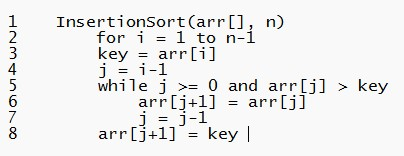
\includegraphics[width=0.8\textwidth,keepaspectratio]{img/insertion.jpg}
		%\includesvg{img/automata.svg}
		%\label{img:mot2}
		%\caption{Product backlog.}
	\end{figure}
	
	\begin{figure}[H]
		\centering
		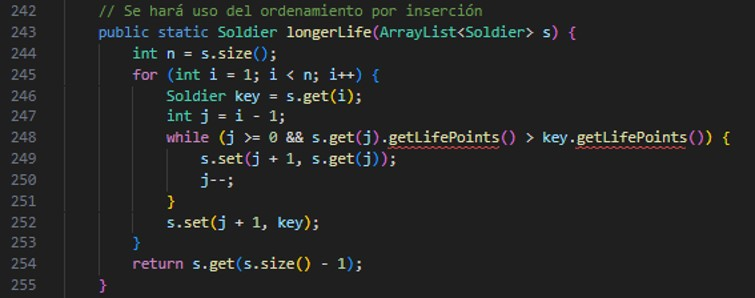
\includegraphics[width=1\textwidth,keepaspectratio]{img/longerLife.jpg}
		%\includesvg{img/automata.svg}
		%\label{img:mot2}
		%\caption{Product backlog.}
	\end{figure}
	
	
	\begin{itemize}	
		\item longerLife(): Se adapta el pseudocódigo de insertion y se le da la forma para que se aplique en un ArrayList. Lo que hace el método es ordenar de menor a mayor, por lo que último elemento es el mayor. El método devuelve al Soldier que se encuentra en esa posición.
		\item Se muestra el pseudocódigo, pero aplicado a un arreglo Estándar. A pesar de ser otra estructura, la idea es la misma
	\end{itemize}
	
	
	\begin{figure}[H]
		\centering
		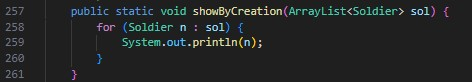
\includegraphics[width=0.99\textwidth,keepaspectratio]{img/showByCreation.jpg}
		%\includesvg{img/automata.svg}
		%\label{img:mot2}
		%\caption{Product backlog.}
	\end{figure}
	
	\begin{itemize}	
		\item showByCreation(): Básicamente imprime los datos de un ArrayList unidimensional de tipo Soldier.
	\end{itemize}
	
	\begin{figure}[H]
		\centering
		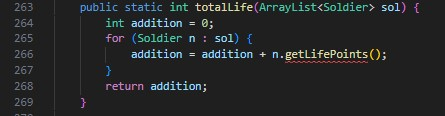
\includegraphics[width=0.99\textwidth,keepaspectratio]{img/totalLife.jpg}
		%\includesvg{img/automata.svg}
		%\label{img:mot2}
		%\caption{Product backlog.}
	\end{figure}	
	
	
	\begin{itemize}	
		\item totalLife(): El método devuelve los puntos de vida total del ejército. Se decide hacer el método con retorno para poder usar esos valores para determinar al ganador y calcular el promedio.
	\end{itemize}
	
	
	
	
	
	\begin{figure}[H]
		\centering
		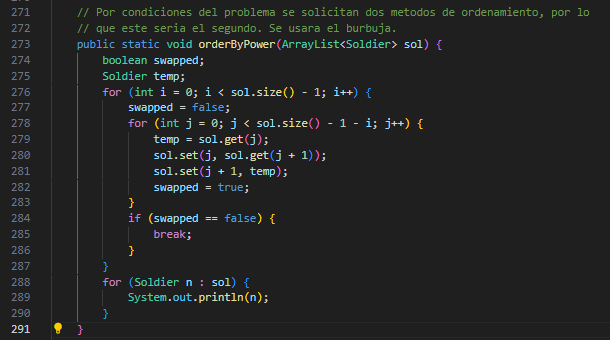
\includegraphics[width=0.98\textwidth,keepaspectratio]{img/orderByPower.png}
		%\includesvg{img/automata.svg}
		%\label{img:mot2}
		%\caption{Product backlog.}
	\end{figure}
	
	\begin{figure}[H]
		\centering
		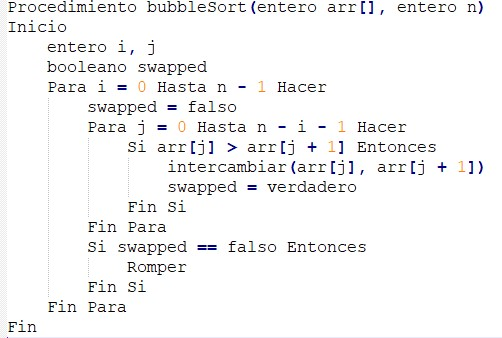
\includegraphics[width=0.9\textwidth,keepaspectratio]{img/burbuja.jpg}
		%\includesvg{img/automata.svg}
		%\label{img:mot2}
		%\caption{Product backlog.}
	\end{figure}
	
	
	\begin{itemize}	
		\item orderByPower(): El método ordena el ArrayList tomando como criterio los puntos de Vida. No se retorna nada
		\item Se muestra el pseudocódigo, pero aplicado a un arreglo Estándar. A pesar de ser otra estructura, la idea es la misma.
	\end{itemize}
	
	\begin{figure}[H]
		\centering
		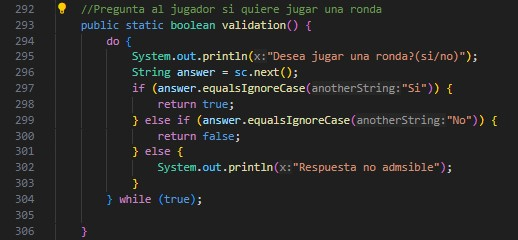
\includegraphics[width=1\textwidth,keepaspectratio]{img/validation.jpg}
		%\includesvg{img/automata.svg}
		%\label{img:mot2}
		%\caption{Product backlog.}
	\end{figure}
	
	\begin{itemize}	
		\item validation(): El método pregunta al usuario si desea jugar una ronda.
	\end{itemize}
	
	\begin{figure}[H]
		\centering
		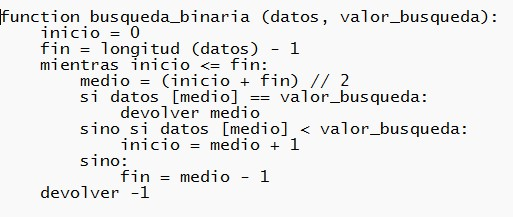
\includegraphics[width=1\textwidth,keepaspectratio]{img/binary.jpg}
		%\includesvg{img/automata.svg}
		%\label{img:mot2}
		%\caption{Product backlog.}
	\end{figure}
	
	
	\begin{itemize}	
		\item Este es el pseudocódigo de búsqueda binaria.
	\end{itemize}
	
	\begin{figure}[H]
		\centering
		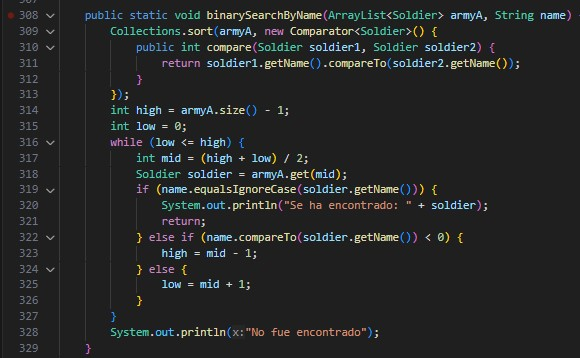
\includegraphics[width=1\textwidth,keepaspectratio]{img/binarySearchByName.jpg}
		%\includesvg{img/automata.svg}
		%\label{img:mot2}
		%\caption{Product backlog.}
	\end{figure}
	

	\begin{itemize}	
		\item La búsqueda binaria será aplicada para buscar por nombres dentro del ArrayList . 
	\end{itemize}
	
	\subsection{Modificación de la clase Soldier}
	
	\begin{lstlisting}[language=bash,caption={Se han aumentado atributos y se crearon tres sobreconstructores sobrecargads }][H]
		code Soldier.java
	\end{lstlisting}
	\begin{figure}[H]
		\centering
		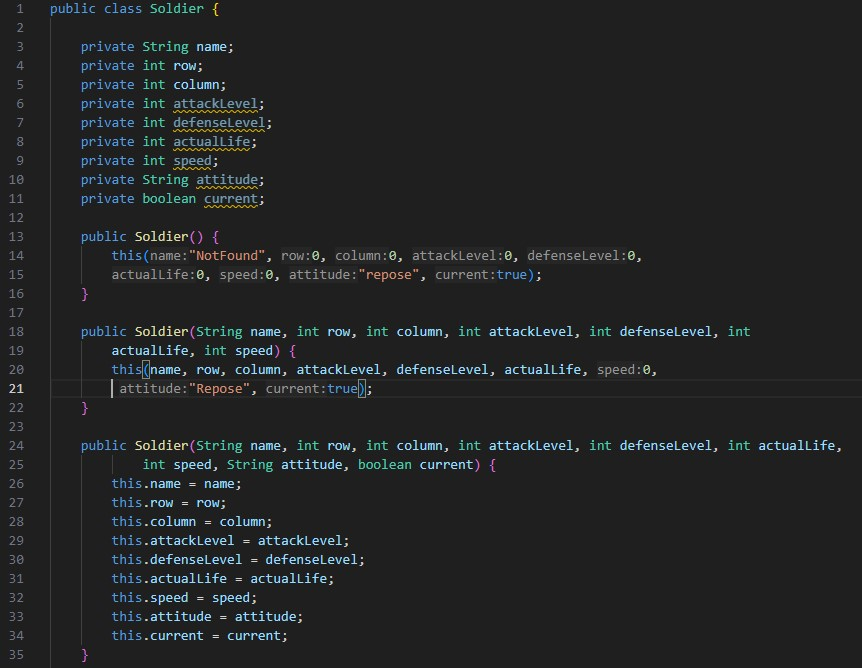
\includegraphics[width=1\textwidth,keepaspectratio]{img/constructors.jpg}
		%\includesvg{img/automata.svg}
		%\label{img:mot2}
		%\caption{Product backlog.}
	\end{figure}
	
	\begin{itemize}	
		\item En una condición de la actividad se nos pedirá usar el método Call Chaining, por lo que al crear un soldier este se iniciará con atributos ya establecidos y ya nos permitirá hacer acciones como sumar los attackLevel por ejemplo. Nos servirá a manera de acumulador.
		\item El segundo es para crear un soldier estableciendo sus atributos desde el main. Este se usará más
		\item El tercero es como plantilla el cual contiene todos los atributos de la clase soldier 
	\end{itemize}
	
	
	\begin{lstlisting}[language=bash,caption={Commit: 59579c7cc3df93a5c893c22138b0b929f99d597e }][H]
		git add Soldier.java
		git commit -m "Se crean los 3 constructores"			
		git push -u origin main
	\end{lstlisting}
	
	
	\begin{lstlisting}[language=bash,caption={Se crean los métodos advance, attack, defend, back, die, beAttacked, scape, getActualLife, setActualLife }][H]
		code Soldier.java
	\end{lstlisting}
	
	\begin{figure}[H]
		\centering
		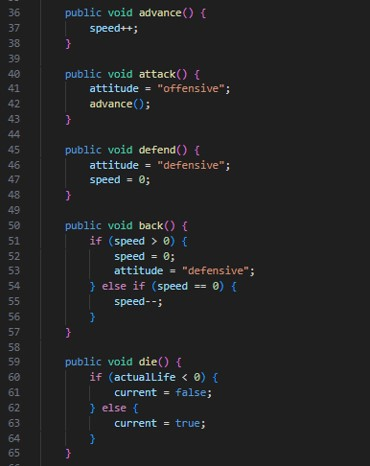
\includegraphics[width=0.8\textwidth,keepaspectratio]{img/method.jpg}
		%\includesvg{img/automata.svg}
		%\label{img:mot2}
		%\caption{Product backlog.}
	\end{figure}
	
	\begin{figure}[H]
		\centering
		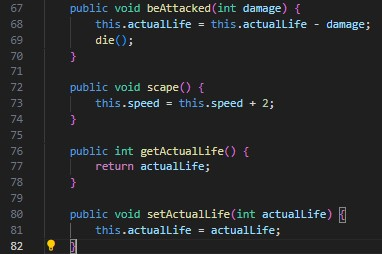
\includegraphics[width=0.8\textwidth,keepaspectratio]{img/method2.jpg}
		%\includesvg{img/automata.svg}
		%\label{img:mot2}
		%\caption{Product backlog.}
	\end{figure}
	
	\begin{figure}[H]
		\centering
		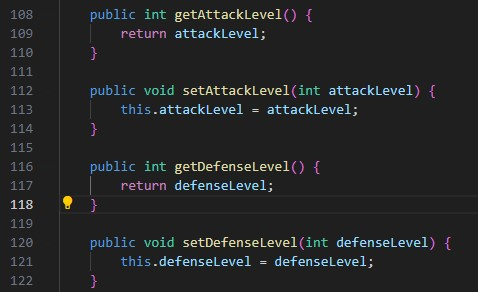
\includegraphics[width=0.8\textwidth,keepaspectratio]{img/method3.jpg}
		%\includesvg{img/automata.svg}
		%\label{img:mot2}
		%\caption{Product backlog.}
	\end{figure}
	
	\begin{figure}[H]
		\centering
		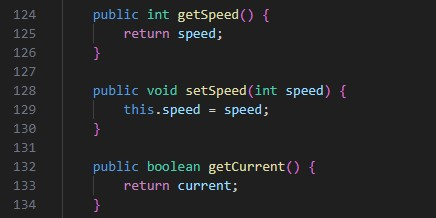
\includegraphics[width=0.8\textwidth,keepaspectratio]{img/method4.jpg}
		%\includesvg{img/automata.svg}
		%\label{img:mot2}
		%\caption{Product backlog.}
	\end{figure}
	
	
	
	\begin{itemize}	
		\item Estos métodos, a pesar de no tener una gran utilidad dentro del videojuego (porque la métrica no se ajusta a los métodos creados ), se nos exige para este laboratorio, además otros se crean con el fin de poder realizar el método de suma de atributos que se verá más adelante . 
	\end{itemize}

	\begin{lstlisting}[language=bash,caption={Commit: 28c2163ac9e7a02e2c83549533267a8c22e28547}][H]
		git add Soldier.java
		git commit -m "Se termina de crear todos los getters y setters"			
		git push -u origin main
	\end{lstlisting}
		
	
	
	
	
	\begin{lstlisting}[language=bash,caption={Se crea el método que clonará la mayoría de atributos de un soldier }][H]
		code Soldier.java
	\end{lstlisting}
	
	\begin{figure}[H]
		\centering
		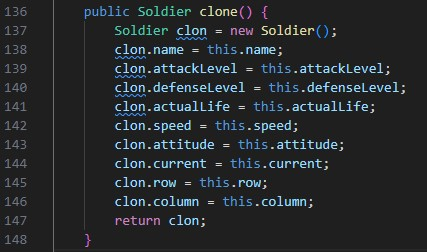
\includegraphics[width=0.9\textwidth,keepaspectratio]{img/clone.jpg}
		%\includesvg{img/automata.svg}
		%\label{img:mot2}
		%\caption{Product backlog.}
	\end{figure}
	
	\begin{itemize}	
		\item Este método clona la mayoría de atributos del soldier que queramos, sin embargo, no se copia los atributos de row y column porque son atributos únicos ya que son la posición del soldier.
	\end{itemize}
	
	\begin{lstlisting}[language=bash,caption={Commit: 614e5b5aae38cf2232af5edb122c0db671195ef5}][H]
		git add Soldier.java
		git commit -m "Metodo que clona un soldier"			
		git push -u origin main
	\end{lstlisting}
	
	
	\begin{lstlisting}[language=bash,caption={El siguiente método comparará atributos }][H]
		code Soldier.java
	\end{lstlisting}
	
	\begin{figure}[H]
		\centering
		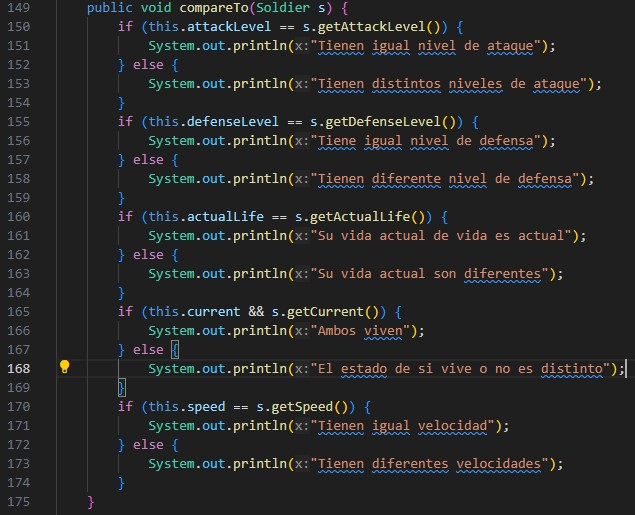
\includegraphics[width=1\textwidth,keepaspectratio]{img/compare.jpg}
		%\includesvg{img/automata.svg}
		%\label{img:mot2}
		%\caption{Product backlog.}
	\end{figure}
	
		
	\begin{lstlisting}[language=bash,caption={Commit: c1eefb734f5354d04097855759507371f7c12d5c}][H]
		git add Soldier.java
		git commit -m "Se crea el metodo comparateTo"			
		git push -u origin main
	\end{lstlisting}
	
	
	
	\begin{lstlisting}[language=bash,caption={Se genera el soldado más poderoso}][H]
		code Soldier.java
	\end{lstlisting}
	
	\begin{figure}[H]
		\centering
		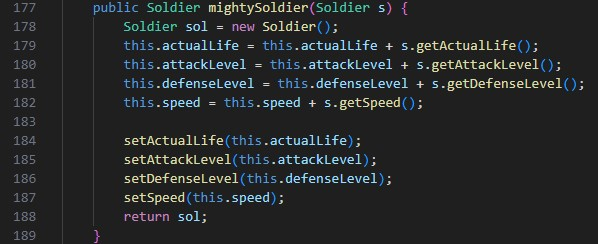
\includegraphics[width=1\textwidth,keepaspectratio]{img/mightySoldier.jpg}
		%\includesvg{img/automata.svg}
		%\label{img:mot2}
		%\caption{Product backlog.}
	\end{figure}
	
	\begin{itemize}	
		\item Este método genera un Soldier con atributos en base a la suma de otros Soldier.
	\end{itemize}
	
	
	\begin{lstlisting}[language=bash,caption={Commit: f813202b9c72f5cefe894fcf22abc6c6f57a3a14}][H]
		git add Soldier.java
		git commit -m "Se corrige el metodo mightySoldier"			
		git push -u origin main
	\end{lstlisting}
	
	
	\begin{lstlisting}[language=bash,caption={Se implementa el método toString}][H]
		code Soldier.java
	\end{lstlisting}
	
	\begin{figure}[H]
		\centering
		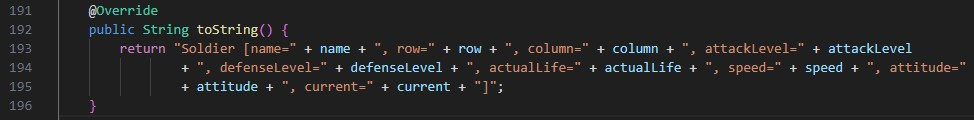
\includegraphics[width=0.8\textwidth,keepaspectratio]{img/toString.jpg}
		%\includesvg{img/automata.svg}
		%\label{img:mot2}
		%\caption{Product backlog.}
	\end{figure}
	
	\begin{lstlisting}[language=bash,caption={Commit: 256779ffb9e686cb971dc63fb7c6ac7fadf36ee1}][H]
		git add Soldier.java
		git commit -m "Se implementa el toString"			
		git push -u origin main
	\end{lstlisting}

	\subsection{Editando VideoJuego.java}
	
	\begin{lstlisting}[language=bash,caption={Se crea un metodo que brinda detalles del enfrentamiento}][H]
		code VideoJuego.java
	\end{lstlisting}
	
	\begin{figure}[H]
		\centering
		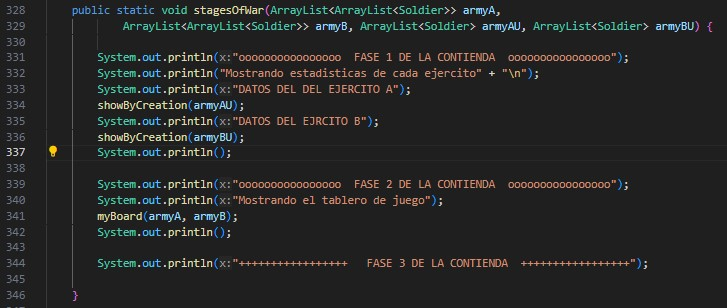
\includegraphics[width=1\textwidth,keepaspectratio]{img/stages.jpg}
		%\includesvg{img/automata.svg}
		%\label{img:mot2}
		%\caption{Product backlog.}
	\end{figure}
	
		
	\begin{itemize}	
		\item Este fragmento de código no es algo nuevo, ya estaba en el main. Ahora se decide incorporarlo a un método para poder rehusarlo ya que el programa nos pedirá iniciar una partida en dos opciones y ya no en una sola como se vino haciendo antes.
	\end{itemize}
	
	
	\begin{lstlisting}[language=bash,caption={Commit: 5818ab3f0158ea7f297ac2415bb32b86f8057596}][H]
		git add VideoJuego.java
		git commit -m "Metodo stagesOfWar pulido"			
		git push -u origin main
	\end{lstlisting}
	
	
	\begin{lstlisting}[language=bash,caption={Se crean arreglos por referencia}][H]
		code VideoJuego.java
	\end{lstlisting}
	
	\begin{figure}[H]
		\centering
		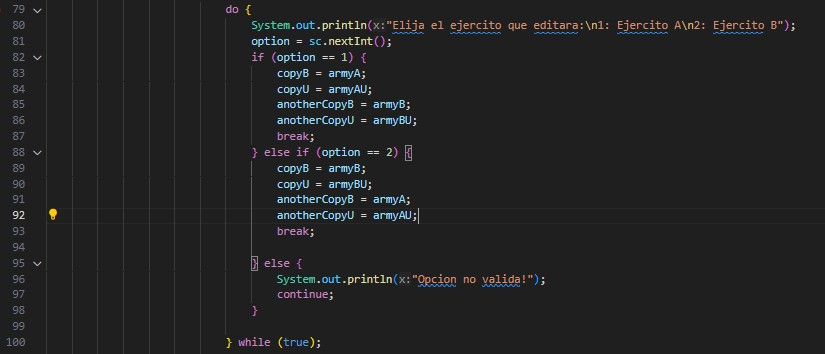
\includegraphics[width=1\textwidth,keepaspectratio]{img/copyReference.jpg}
		%\includesvg{img/automata.svg}
		%\label{img:mot2}
		%\caption{Product backlog.}
	\end{figure}
	
	
	\begin{itemize}	
		\item En el main, hasta este punto se realizó un bosquejo del flujo del programa, sin embargo, lo más importante es este fragmento de código el cual nos permite inicializar ArrayList usando referencia, esto con el fin de poder realizar cambios en los ArrayList originales.
	\end{itemize}
	
	\begin{lstlisting}[language=bash,caption={Commit: 5ae36c4b0202868075638aae95cc8a9a36f36118}][H]
		git add VideoJuego.java
		git commit -m "Se crean arreglos por referencia"			
		git push -u origin main
	\end{lstlisting}	
	
	
	
	\begin{lstlisting}[language=bash,caption={Metodo que trasnforma ArrayList Bidimensioanles a Unidimensionales}][H]
		code VideoJuego.java
	\end{lstlisting}
	
	\begin{figure}[H]
		\centering
		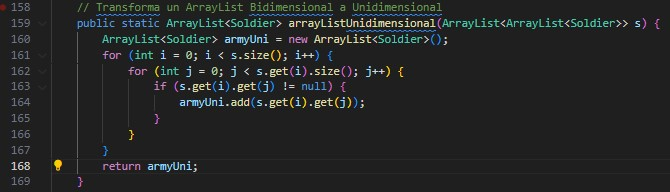
\includegraphics[width=1\textwidth,keepaspectratio]{img/arrayListU.jpg}
		%\includesvg{img/automata.svg}
		%\label{img:mot2}
		%\caption{Product backlog.}
	\end{figure}
	
	
	\begin{itemize}	
		\item Este método sirve para poder trabajar de manera más sencilla con otros métodos como binarySearch entre otros.
	\end{itemize}
	
	
	
	
	
	
	
	
	
	
	
	\begin{lstlisting}[language=bash,caption={Se crea un método que iniciliza elementos de un ArrayList con nulls}][H]
		code VideoJuego.java
	\end{lstlisting}
	
	\begin{figure}[H]
		\centering
		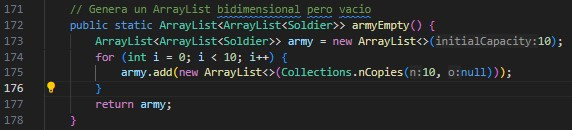
\includegraphics[width=1\textwidth,keepaspectratio]{img/armyEmpty.jpg}
		%\includesvg{img/automata.svg}
		%\label{img:mot2}
		%\caption{Product backlog.}
	\end{figure}
	
	
	\begin{itemize}	
		\item Este método genera llena ArrayList con nulls con el fin de servir como apoyo al momento de inicializar los ArrayList con objetos del tipo Soldier sin generar repeticiones.
	\end{itemize}
	

	
	\begin{lstlisting}[language=bash,caption={Commit: 55bd8cf312296a9a1727dc08824c0de7936e5060}][H]
		git add VideoJuego.java
		git commit -m "Metodo que genera un ArrayList bidimensional vacio"			
		git push -u origin main
	\end{lstlisting}	
	

	
	
	
	
	\begin{lstlisting}[language=bash,caption={Método que transforma ArrayList bidimensioanles en unidimensionales}][H]
		code VideoJuego.java
	\end{lstlisting}
	
	\begin{figure}[H]
		\centering
		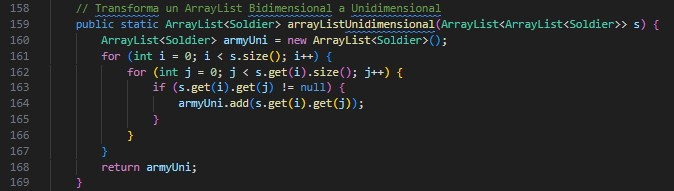
\includegraphics[width=1\textwidth,keepaspectratio]{img/generateUni.jpg}
		%\includesvg{img/automata.svg}
		%\label{img:mot2}
		%\caption{Product backlog.}
	\end{figure}
	
		
	\begin{itemize}	
		\item arrayListUnidimensional: A pesar de ya contar con dos ArrayList bidimensionales, se opta por transformarlos en ArrayList unidimensionales ya que nos facilitará trabajar con los demás métodos que la práctica de laboratorio solicita. En el main se hace la creación de dos ArrayList unidimensionales tanto para el ejército A y B. Este método ya se venía presentando en laboratorios anteriores, por lo que no sufrió alteraciones.
	\end{itemize}
	
	
	
	\begin{lstlisting}[language=bash,caption={Se mejora el método que permite iniciliazar los ArrayList con objetos de tipo soldier. }][H]
		code VideoJuego.java
	\end{lstlisting}
	
	\begin{figure}[H]
		\centering
		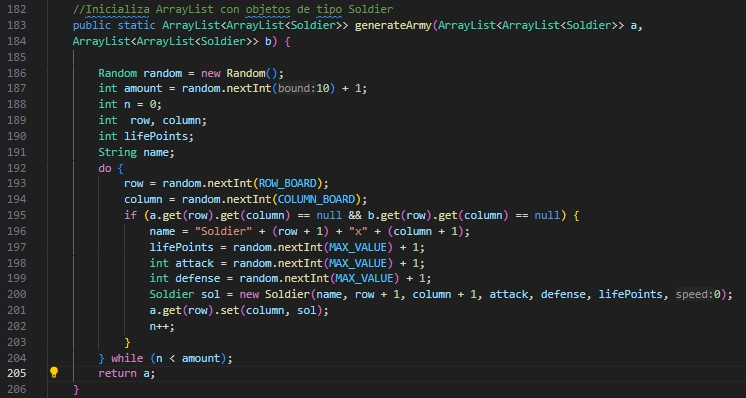
\includegraphics[width=1\textwidth,keepaspectratio]{img/generateArmy.jpg}
		%\includesvg{img/automata.svg}
		%\label{img:mot2}
		%\caption{Product backlog.}
	\end{figure}
	
	
	\begin{itemize}	
		\item Este método genera objetos de tipo Soldier bien definidos y los guarda en un ArrayList. Se usan constantes de clases para generar los atributos de cada soldier. Básicamente, para el llenado de objetos para ambos ejércitos, la primera vez que se lo invoca, se pasan como parámetros dos ArrayList vacíos, para generarel segundo ejército se le manda un ArrayList vacío y el que hemos llenado con el uso de este método (el primer ArrayLis que se llenó). 
	\end{itemize}
	
	\begin{lstlisting}[language=bash,caption={Commit: d4f69f7ac1e9eaddbdca6dae2b5b253ebfcce269}][H]
		git add VideoJuego.java
		git commit -m "Se mejora el metodo generateArmy"			
		git push -u origin main
	\end{lstlisting}	
	
	
	
	
	
	\begin{lstlisting}[language=bash,caption={Se hacen cambios en el método myBoard }][H]
		code VideoJuego.java
	\end{lstlisting}
	
	\begin{figure}[H]
		\centering
		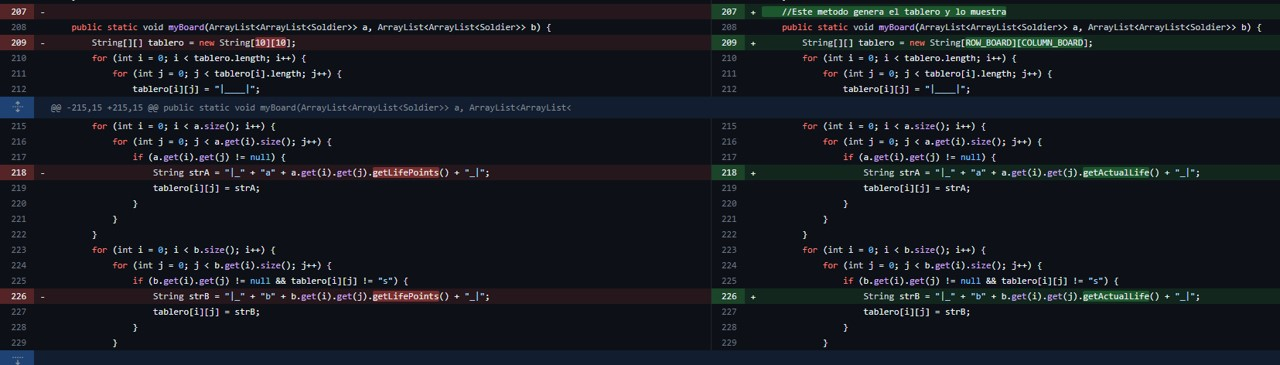
\includegraphics[width=1\textwidth,keepaspectratio]{img/changesMyBoard.jpg}
		%\includesvg{img/automata.svg}
		%\label{img:mot2}
		%\caption{Product backlog.}
	\end{figure}
	
	
	\begin{itemize}	
		\item La lógica con la que el tablero se genera y se muestra no se alteró, sin embargo, se optó por usar las constantes de clases para evitar "números fantasmas", además se cambia el método getLifePoints por getActualLifePoints.
	\end{itemize}
	
	\begin{figure}[H]
		\centering
		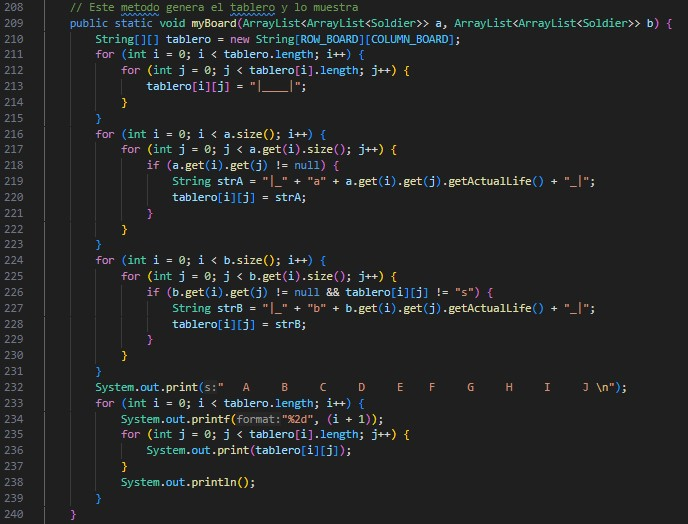
\includegraphics[width=1\textwidth,keepaspectratio]{img/myBoard.jpg}
		%\includesvg{img/automata.svg}
		%\label{img:mot2}
		%\caption{Product backlog.}
	\end{figure}
	
	\begin{itemize}	
		\item Aquí se muestra el método myBoard de forma completa.
	\end{itemize}
		
	\begin{lstlisting}[language=bash,caption={Commit: a0f41647ec8dad5414cdd80eeac576c145bc032f}][H]
		git add VideoJuego.java
		git commit -m "Se modifican algunas cosas dentro del tablero"			
		git push -u origin main
	\end{lstlisting}	




	\begin{lstlisting}[language=bash,caption={Se implementa el método que recibe una coordenada }][H]
		code VideoJuego.java
	\end{lstlisting}
	
	\begin{figure}[H]
		\centering
		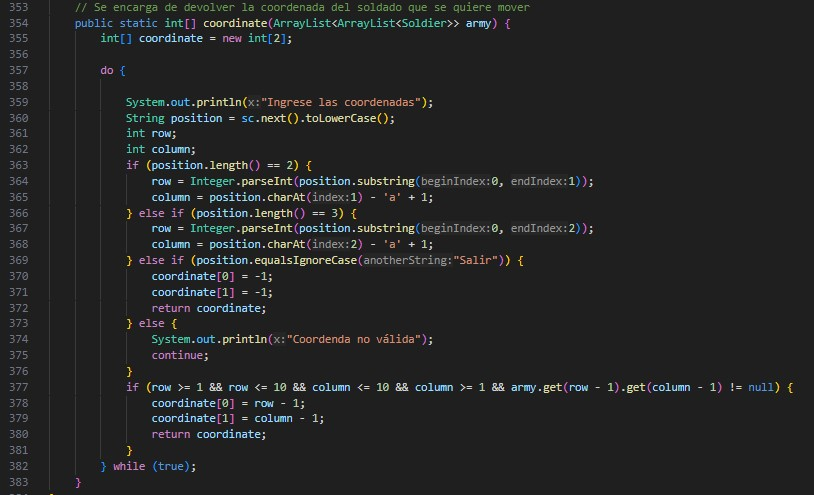
\includegraphics[width=1\textwidth,keepaspectratio]{img/coordinate.jpg}
		%\includesvg{img/automata.svg}
		%\label{img:mot2}
		%\caption{Product backlog.}
	\end{figure}
	
	
	\begin{itemize}	
		\item Este método sirve para que el usuario ingrese una coordenda (por ejemplo 1A), desglosando así el String en números enteros que representan la fila y columna (Ejm: 0 y 0 es el resultado de ingresar 1A, dichos valores son procesados por los demás métodos).
	\end{itemize}
	
	\begin{lstlisting}[language=bash,caption={Commit: 0350a4047a04c3909a8829c31ee143472164c509}][H]
		git add VideoJuego.java
		git commit -m "Se crea el coordinate"			
		git push -u origin main
	\end{lstlisting}
	


	\begin{lstlisting}[language=bash,caption={Se implementa el método que da una dirección de movimiento }][H]
		code VideoJuego.java
	\end{lstlisting}
	
	\begin{figure}[H]
		\centering
		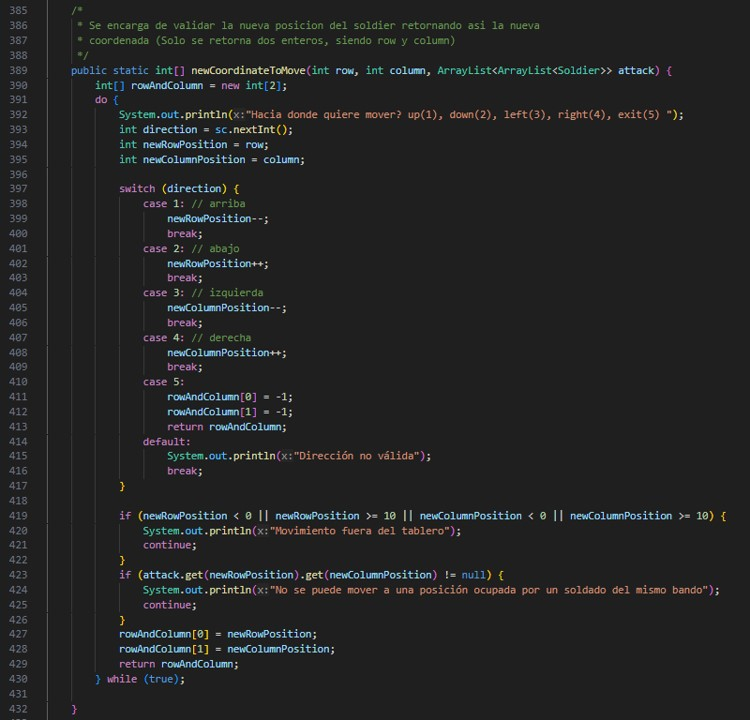
\includegraphics[width=1\textwidth,keepaspectratio]{img/newCoordinate.jpg}
		%\includesvg{img/automata.svg}
		%\label{img:mot2}
		%\caption{Product backlog.}
	\end{figure}
	
	
	\begin{itemize}	
		\item Este método sirve para que el soldier pueda moverse a una determinada posición (arriba, abajo, izquierda, derecha). Retorna un arreglo que contiene la nueva coordenada donde el soldier deberá moverse.
	\end{itemize}
	
	\begin{lstlisting}[language=bash,caption={Commit: ae376e9c6b501f2d37a8979eb6f488a5b4ce4890}][H]
		git add VideoJuego.java
		git commit -m "Se crea el metodo newCoordinateToMove"			
		git push -u origin main
	\end{lstlisting}
	


	\begin{lstlisting}[language=bash,caption={Se implementa el método que mueve al Soldier a otra casilla}][H]
		code VideoJuego.java
	\end{lstlisting}
	
	\begin{figure}[H]
		\centering
		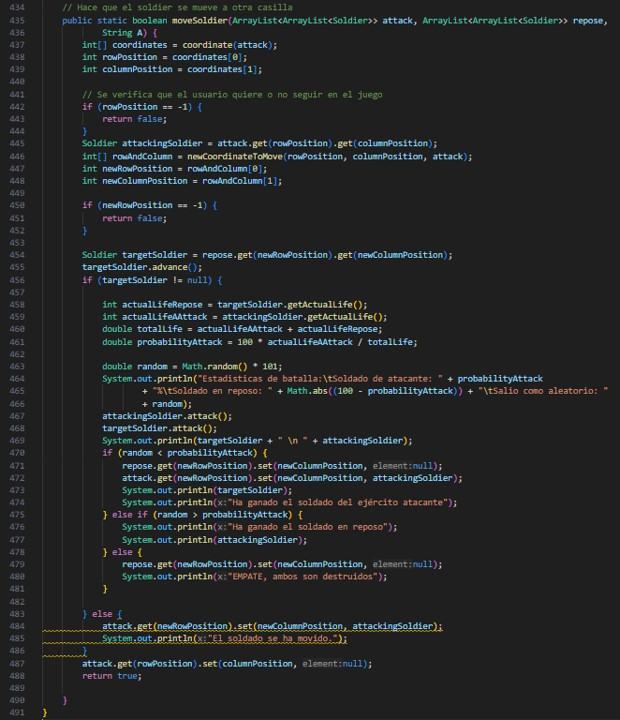
\includegraphics[width=1\textwidth,keepaspectratio]{img/moveSoldier.jpg}
		%\includesvg{img/automata.svg}
		%\label{img:mot2}
		%\caption{Product backlog.}
	\end{figure}
	
	
	\begin{itemize}	
		\item Este método usa los métodos coordinate y newCoordinateToMove para hacer el desplazamiento corespondiente, para ello tenemos dos casos principales. El primero es que el soldier a mover no tenga cruces con un soldier del equipo rival, el segundo caso es que haya cruce y por ende se ocasione una batalla y en esta parte se implementa la lógica de enfrentamiento, la cual consiste en generar un número aleatorio que debe estar entre el rango de la probabilidad que tiene cada soldier de ganar que se calcula en base de la vida actual, por ejemplo si el Soldier A tiene 2 y el Soldier B tiene 4, la probabilidad de A es 33.3 y la de B es de 66.6, por lo que si el aletorio es de 27.7, ganaría el ejército A.
	\end{itemize}
	
	\begin{lstlisting}[language=bash,caption={Commit: aa83f83f4aac63d6a92bb824f0dab2411cbb886f}][H]
		git add VideoJuego.java
		git commit -m "Se crea el metodo moveSoldier"			
		git push -u origin main
	\end{lstlisting}
	
	
	\begin{lstlisting}[language=bash,caption={Se implementa el método que verifica si queda algún objeto dentro de un ArrayList }][H]
		code VideoJuego.java
	\end{lstlisting}
	
	\begin{figure}[H]
		\centering
		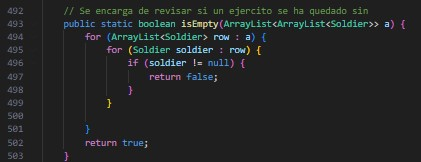
\includegraphics[width=1\textwidth,keepaspectratio]{img/isEmpty.jpg}
		%\includesvg{img/automata.svg}
		%\label{img:mot2}
		%\caption{Product backlog.}
	\end{figure}
	
	
	\begin{itemize}	
		\item Este método se encarga de verificar si aún quedan objetos dentro del ArrayList, más adelante se complementará con otros métodos que dictaminarán al ganador de la contienda.
	\end{itemize}
	
	\begin{lstlisting}[language=bash,caption={Commit: ab3d57e656981530cd4e74610edf81c1cc600f95}][H]
		git add VideoJuego.java
		git commit -m "Se crea el metodo isEmpty"			
		git push -u origin main
	\end{lstlisting}
	
	
	
	\begin{lstlisting}[language=bash,caption={Se implementa el método que determina al ganador }][H]
		code VideoJuego.java
	\end{lstlisting}
	
	\begin{figure}[H]
		\centering
		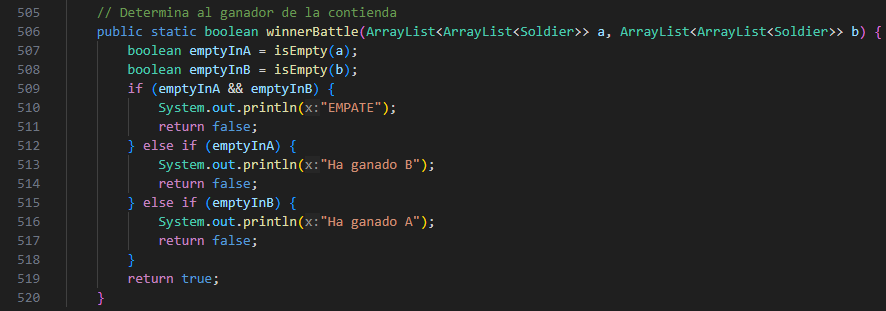
\includegraphics[width=1\textwidth,keepaspectratio]{img/winnerBattle.png}
		%\includesvg{img/automata.svg}
		%\label{img:mot2}
		%\caption{Product backlog.}
	\end{figure}
	
	
	\begin{itemize}	
		\item Este método se encarga de verificar si aún quedan objetos dentro del ArrayList, más adelante se complementará con otros método que dictaminarán al ganador de la contienda.
	\end{itemize}
	
	\begin{lstlisting}[language=bash,caption={Commit: 04134f5051779fbd5b19cbea7b9a076d56d46d90}][H]
		git add VideoJuego.java
		git commit -m "Se crea el metodo el metodo winnerBattle"			
		git push -u origin main
	\end{lstlisting}
	
	
	\begin{lstlisting}[language=bash,caption={Se implementa el método para crear un Soldier }][H]
		code VideoJuego.java
	\end{lstlisting}
	
	\begin{figure}[H]
		\centering
		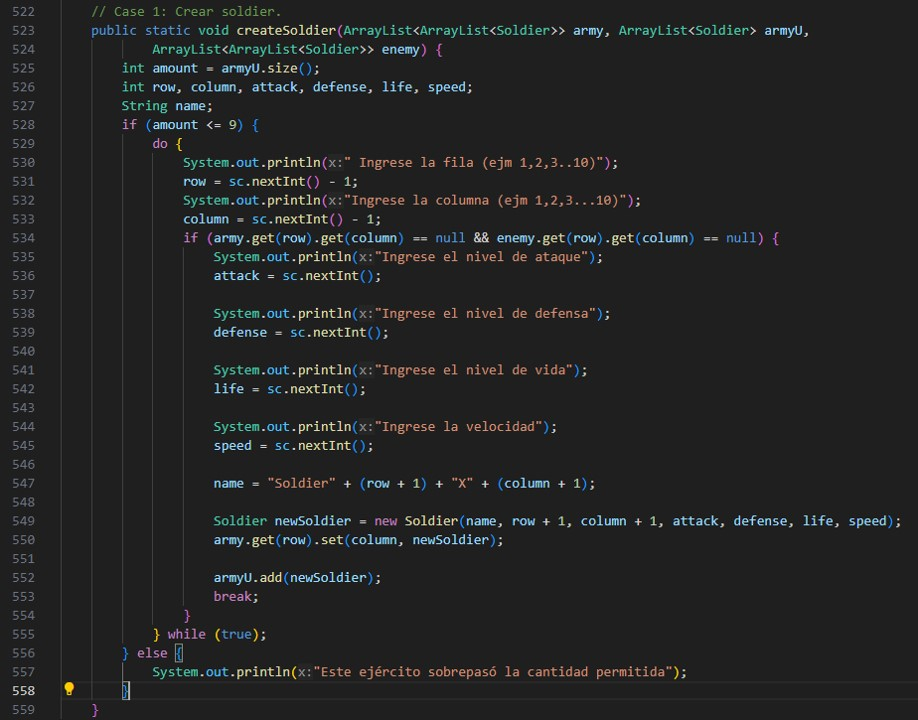
\includegraphics[width=1\textwidth,keepaspectratio]{img/createSoldier.jpg}
		%\includesvg{img/automata.svg}
		%\label{img:mot2}
		%\caption{Product backlog.}
	\end{figure}
	
	
	\begin{itemize}	
		\item Este método se encarga de crear un nuevo Soldier sin que sobrepase la capacidad máxima establecida.
	\end{itemize}
	
	
	\begin{lstlisting}[language=bash,caption={Compilando y probando}][H]
		javac VideoJuego.java
		java VideoJuego
		1: Juego rapido
		2: Juego personalizado
		3: Salir
		2
		DATOS DEL EJRCITO A
		Soldier [name=Soldier2x6, lifePoints=, row=2, column=6]
		Soldier [name=Soldier8x7, lifePoints=, row=8, column=7]
		DATOS DEL EJRCITO B
		Soldier [name=Soldier2x4, lifePoints=, row=2, column=4]
		Soldier [name=Soldier3x9, lifePoints=, row=3, column=9]
		Soldier [name=Soldier5x7, lifePoints=, row=5, column=7]
		Soldier [name=Soldier6x7, lifePoints=, row=6, column=7]
		Soldier [name=Soldier8x8, lifePoints=, row=8, column=8]
		Soldier [name=Soldier9x3, lifePoints=, row=9, column=3]
		1: Crear soldado
		2: Eliminar soldado
		3: Clonar soldado
		4: Modificar soldado
		5: Comparar Soldado
		6: Intercambiar soldado
		7: Ver soldado
		8: Ver ejercito
		9: Sumar niveles
		10: Jugar
		11: Volver al menu principal
		1
		Elija el ejercito que editara:
		1: Ejercito A
		2: Ejercito B
		1
		Ingrese la fila (ejm 1,2,3..10)
		1
		Ingrese la columna (ejm 1,2,3...10)
		1
		Ingrese el nivel de ataque
		5
		Ingrese el nivel de defensa
		5
		Ingrese el nivel de vida
		5
		Ingrese la velocidad
		5
		DATOS DEL EJRCITO A
		Soldier [name=Soldier2x6, lifePoints=, row=2, column=6]
		Soldier [name=Soldier8x7, lifePoints=, row=8, column=7]
		Soldier [name=Soldier1X1, lifePoints=, row=1, column=1]
		DATOS DEL EJRCITO B
		Soldier [name=Soldier2x4, lifePoints=, row=2, column=4]
		Soldier [name=Soldier3x9, lifePoints=, row=3, column=9]
		Soldier [name=Soldier5x7, lifePoints=, row=5, column=7]
		Soldier [name=Soldier6x7, lifePoints=, row=6, column=7]
		Soldier [name=Soldier8x8, lifePoints=, row=8, column=8]
		Soldier [name=Soldier9x3, lifePoints=, row=9, column=3]
		1: Crear soldado
		2: Eliminar soldado
		3: Clonar soldado
		4: Modificar soldado
		5: Comparar Soldado
		6: Intercambiar soldado
		7: Ver soldado
		8: Ver ejercito
		9: Sumar niveles
		10: Jugar
		11: Volver al menu principal
		11
		1: Juego rapido
		2: Juego personalizado
		3: Salir
		3
	\end{lstlisting}
	
	\begin{itemize}	
		\item Se está probando el menú y la opción de crear Soldier.
	\end{itemize}
	
	\begin{lstlisting}[language=bash,caption={Commit: 0802334d8d151230f14cdf4a1e05ecbccf6f5738}][H]
		git add VideoJuego.java
		git commit -m "Se crea el metodo createSoldier"			
		git push -u origin main
	\end{lstlisting}
	
	
	
	
	
	\begin{lstlisting}[language=bash,caption={Se implementa el método para eliminar un Soldier }][H]
		code VideoJuego.java
	\end{lstlisting}
	
	\begin{figure}[H]
		\centering
		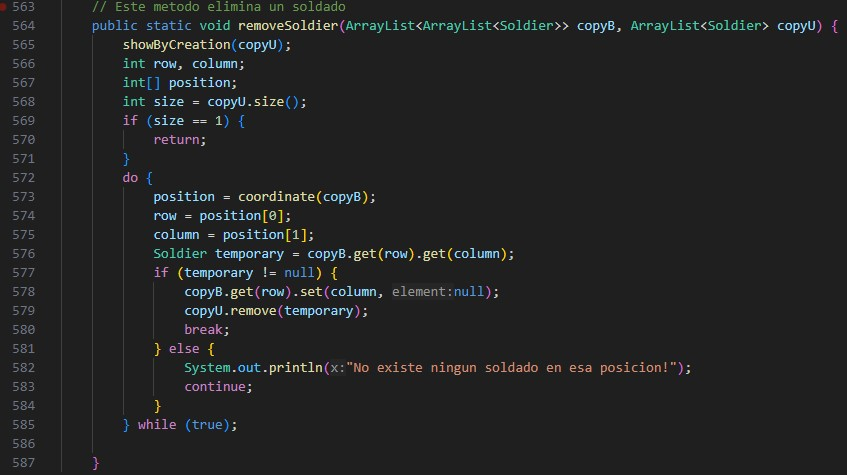
\includegraphics[width=1\textwidth,keepaspectratio]{img/removeSoldier.jpg}
		%\includesvg{img/automata.svg}
		%\label{img:mot2}
		%\caption{Product backlog.}
	\end{figure}
	
	
	\begin{itemize}	
		\item Este método se encarga de borrar un Soldier, la acción no se ejecutará si el ejército tiene como máximo un elemento.
	\end{itemize}
	
	
	\begin{lstlisting}[language=bash,caption={Compilando y probando el método removeSoldier  }][H]
	javac VideoJuego.java
	java VideoJuego
	1: Juego rapido
	2: Juego personalizado
	3: Salir
	2
	DATOS DEL EJRCITO A
	Soldier [name=Soldier10x7, lifePoints=, row=10, column=7]
	DATOS DEL EJRCITO B
	Soldier [name=Soldier5x7, lifePoints=, row=5, column=7]
	Soldier [name=Soldier8x3, lifePoints=, row=8, column=3]
	1: Crear soldado
	2: Eliminar soldado
	3: Clonar soldado
	4: Modificar soldado
	5: Comparar Soldado
	6: Intercambiar soldado
	7: Ver soldado
	8: Ver ejercito
	9: Sumar niveles
	10: Jugar
	11: Volver al menu principal
	2
	Elija el ejercito que editara:
	1: Ejercito A
	2: Ejercito B
	2
	Debe Eliminar un soldado
		A      B       C     D     E      F     G      H     I     J
	1 |____||____||____||____||____||____||____||____||____||____|
	2 |____||____||____||____||____||____||____||____||____||____|
	3 |____||____||____||____||____||____||____||____||____||____|
	4 |____||____||____||____||____||____||____||____||____||____|
	5 |____||____||____||____||____||____||_b2_||____||____||____|
	6 |____||____||____||____||____||____||____||____||____||____|
	7 |____||____||____||____||____||____||____||____||____||____|
	8 |____||____||_b2_||____||____||____||____||____||____||____|
	9 |____||____||____||____||____||____||____||____||____||____|
	10|____||____||____||____||____||____||_a2_||____||____||____|
	Soldier [name=Soldier5x7, lifePoints=, row=5, column=7]
	Soldier [name=Soldier8x3, lifePoints=, row=8, column=3]
	Ingrese las coordenadas
	8c
	DATOS DEL EJRCITO A
	Soldier [name=Soldier10x7, lifePoints=, row=10, column=7]
	DATOS DEL EJRCITO B
	Soldier [name=Soldier5x7, lifePoints=, row=5, column=7]
	1: Crear soldado
	2: Eliminar soldado
	3: Clonar soldado
	4: Modificar soldado
	5: Comparar Soldado
	6: Intercambiar soldado
	7: Ver soldado
	8: Ver ejercito
	9: Sumar niveles
	10: Jugar
	11: Volver al menu principal
	11
	1: Juego rapido
	2: Juego personalizado
	3: Salir
	3
	\end{lstlisting}
	

	\begin{lstlisting}[language=bash,caption={Commit: 28886c9cee9a351810f14da8769e1c922a221904}][H]
		git add VideoJuego.java
		git commit -m "Se crea el metodo removeSoldier"			
		git push -u origin main
	\end{lstlisting}
	
	
	
	
	
	\begin{lstlisting}[language=bash,caption={Se implementa el método para clonar un soldado }][H]
		code VideoJuego.java
	\end{lstlisting}
	
	\begin{figure}[H]
		\centering
		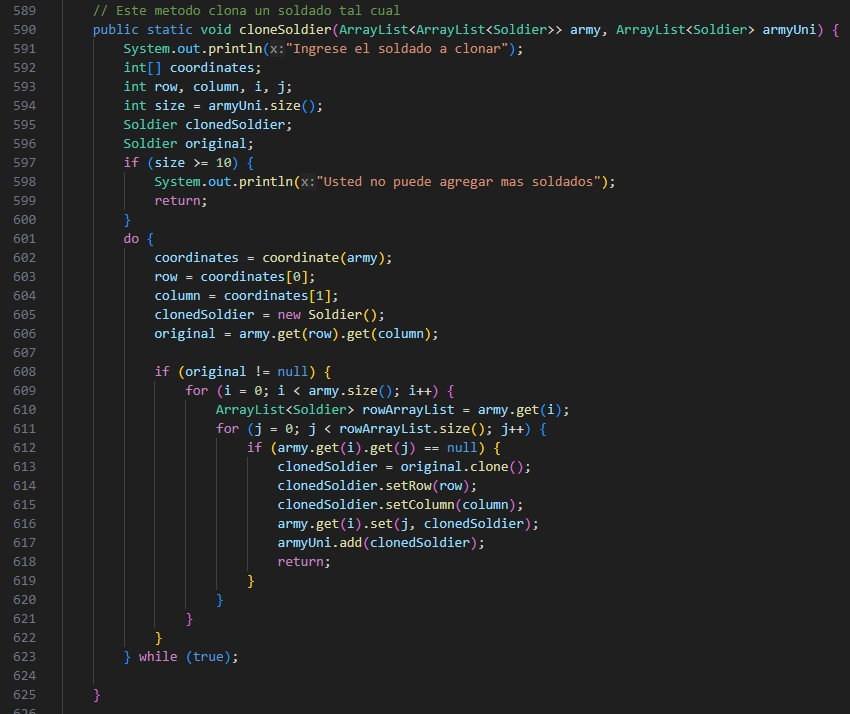
\includegraphics[width=1\textwidth,keepaspectratio]{img/cloneSoldier.jpg}
		%\includesvg{img/automata.svg}
		%\label{img:mot2}
		%\caption{Product backlog.}
	\end{figure}
	
	
	\begin{itemize}	
		\item Este método se encarga de clonar un Soldier, la acción no se ejecutará si el ejército tiene 10 objetos. Para lograr este propósito, se hace uso del método de la clase Soldier clone el cual ya fue explicado. A pesar de que el método debe clonar un Soldier tal cual, no se llega a cumplir a cabalidad ya que los atributos de row y column son únicos puesto que son la ubicación del soldier.
	\end{itemize}
	
	
	\begin{lstlisting}[language=bash,caption={Compilando y probando el metodo cloneSoldier  }][H]
	javac VideoJuego.java
	java VideoJuego
	1: Juego rapido
	2: Juego personalizado
	3: Salir
	2
	DATOS DEL EJRCITO A
	Soldier [name=Soldier2x4, lifePoints=, row=2, column=4]
	Soldier [name=Soldier2x8, lifePoints=, row=2, column=8]
	Soldier [name=Soldier3x5, lifePoints=, row=3, column=5]
	Soldier [name=Soldier6x1, lifePoints=, row=6, column=1]
	Soldier [name=Soldier6x3, lifePoints=, row=6, column=3]
	Soldier [name=Soldier7x9, lifePoints=, row=7, column=9]
	DATOS DEL EJRCITO B
	Soldier [name=Soldier1x1, lifePoints=, row=1, column=1]
	Soldier [name=Soldier2x3, lifePoints=, row=2, column=3]
	Soldier [name=Soldier4x6, lifePoints=, row=4, column=6]
	Soldier [name=Soldier5x4, lifePoints=, row=5, column=4]
	Soldier [name=Soldier6x7, lifePoints=, row=6, column=7]
	Soldier [name=Soldier7x6, lifePoints=, row=7, column=6]
	Soldier [name=Soldier8x7, lifePoints=, row=8, column=7]
	Soldier [name=Soldier9x2, lifePoints=, row=9, column=2]
	1: Crear soldado
	2: Eliminar soldado
	3: Clonar soldado
	4: Modificar soldado
	5: Comparar Soldado
	6: Intercambiar soldado
	7: Ver soldado
	8: Ver ejercito
	9: Sumar niveles
	10: Jugar
	11: Volver al menu principal
	3
	Elija el ejercito que editara:
	1: Ejercito A
	2: Ejercito B
	1
	Ingrese el soldado a clonar
	Ingrese las coordenadas
	6a
	DATOS DEL EJRCITO A
	Soldier [name=Soldier2x4, lifePoints=, row=2, column=4]
	Soldier [name=Soldier2x8, lifePoints=, row=2, column=8]
	Soldier [name=Soldier3x5, lifePoints=, row=3, column=5]
	Soldier [name=Soldier6x1, lifePoints=, row=6, column=1]
	Soldier [name=Soldier6x3, lifePoints=, row=6, column=3]
	Soldier [name=Soldier7x9, lifePoints=, row=7, column=9]
	Soldier [name=Soldier6x1, lifePoints=, row=5, column=0]
	DATOS DEL EJRCITO B
	Soldier [name=Soldier1x1, lifePoints=, row=1, column=1]
	Soldier [name=Soldier2x3, lifePoints=, row=2, column=3]
	Soldier [name=Soldier4x6, lifePoints=, row=4, column=6]
	Soldier [name=Soldier5x4, lifePoints=, row=5, column=4]
	Soldier [name=Soldier6x7, lifePoints=, row=6, column=7]
	Soldier [name=Soldier7x6, lifePoints=, row=7, column=6]
	Soldier [name=Soldier8x7, lifePoints=, row=8, column=7]
	Soldier [name=Soldier9x2, lifePoints=, row=9, column=2]
	1: Crear soldado
	2: Eliminar soldado
	3: Clonar soldado
	4: Modificar soldado
	5: Comparar Soldado
	6: Intercambiar soldado
	7: Ver soldado
	8: Ver ejercito
	9: Sumar niveles
	10: Jugar
	11: Volver al menu principal
	11
	1: Juego rapido
	2: Juego personalizado
	3: Salir
	3
	\end{lstlisting}
	
	
	\begin{lstlisting}[language=bash,caption={Commit: c98829adbf11f4704c7b2950873e39e70603d38d}][H]
		git add VideoJuego.java
		git commit -m "Se crea el metodo cloneSoldier"			
		git push -u origin main
	\end{lstlisting}
	
	
	
	
	\begin{lstlisting}[language=bash,caption={Se implementa el método para cambiar los atributos de un soldado }][H]
		code VideoJuego.java
	\end{lstlisting}
	
	\begin{figure}[H]
		\centering
		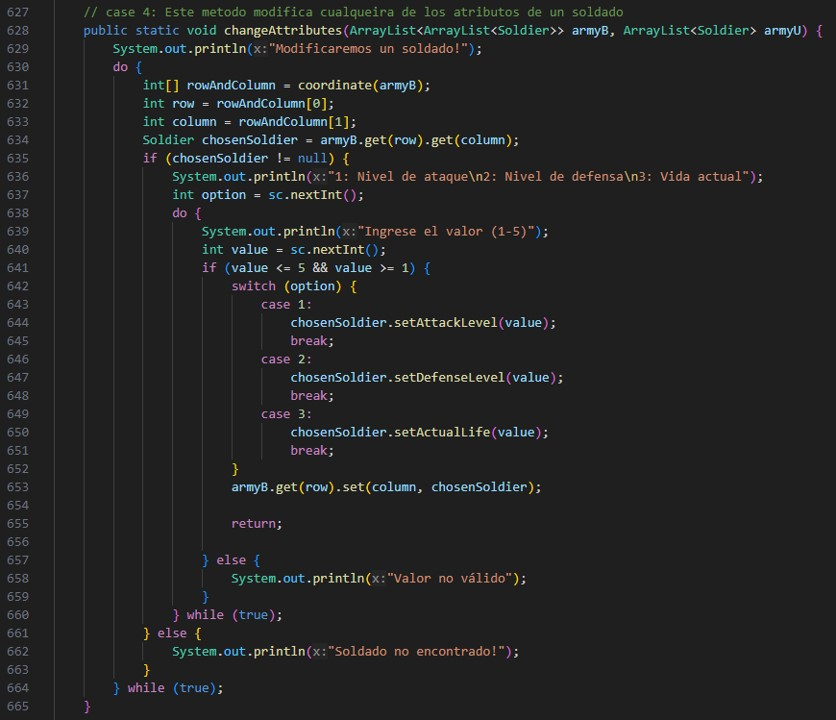
\includegraphics[width=1\textwidth,keepaspectratio]{img/changeAttribute.jpg}
		%\includesvg{img/automata.svg}
		%\label{img:mot2}
		%\caption{Product backlog.}
	\end{figure}
	
	\begin{itemize}	
		\item Este método se encarga de modificar los atributos de un Soldier, entre estos tenemos el nivel de vida actual, los puntos de ataque y defensa.
	\end{itemize}
	
	\begin{lstlisting}[language=bash,caption={Compilando y probando el metodo changeAttribute  }][H]
		javac VideoJuego.java
		java VideoJuego
		1: Juego rapido
		2: Juego personalizado
		3: Salir
		2
		DATOS DEL EJRCITO A
		Soldier [name=Soldier1x10, row=1, column=10, attackLevel=3, defenseLevel=1, actualLife=2, speed=0, attitude=Repose, current=true]
		Soldier [name=Soldier2x7, row=2, column=7, attackLevel=1, defenseLevel=5, actualLife=1, speed=0, attitude=Repose, current=true]
		Soldier [name=Soldier3x2, row=3, column=2, attackLevel=1, defenseLevel=2, actualLife=2, speed=0, attitude=Repose, current=true]
		Soldier [name=Soldier4x8, row=4, column=8, attackLevel=1, defenseLevel=2, actualLife=3, speed=0, attitude=Repose, current=true]
		Soldier [name=Soldier5x7, row=5, column=7, attackLevel=3, defenseLevel=2, actualLife=1, speed=0, attitude=Repose, current=true]
		Soldier [name=Soldier5x9, row=5, column=9, attackLevel=1, defenseLevel=4, actualLife=1, speed=0, attitude=Repose, current=true]
		Soldier [name=Soldier8x6, row=8, column=6, attackLevel=3, defenseLevel=5, actualLife=4, speed=0, attitude=Repose, current=true]
		Soldier [name=Soldier8x8, row=8, column=8, attackLevel=2, defenseLevel=5, actualLife=3, speed=0, attitude=Repose, current=true]
		Soldier [name=Soldier9x2, row=9, column=2, attackLevel=3, defenseLevel=1, actualLife=4, speed=0, attitude=Repose, current=true]
		Soldier [name=Soldier9x9, row=9, column=9, attackLevel=2, defenseLevel=5, actualLife=2, speed=0, attitude=Repose, current=true]
		DATOS DEL EJRCITO B
		Soldier [name=Soldier1x2, row=1, column=2, attackLevel=3, defenseLevel=4, actualLife=4, speed=0, attitude=Repose, current=true]
		Soldier [name=Soldier4x4, row=4, column=4, attackLevel=2, defenseLevel=1, actualLife=5, speed=0, attitude=Repose, current=true]
		Soldier [name=Soldier7x9, row=7, column=9, attackLevel=4, defenseLevel=2, actualLife=1, speed=0, attitude=Repose, current=true]
		1: Crear soldado
		2: Eliminar soldado
		3: Clonar soldado
		4: Modificar soldado
		5: Comparar Soldado
		6: Intercambiar soldado
		7: Ver soldado
		8: Ver ejercito
		9: Sumar niveles
		10: Jugar
		11: Volver al menu principal
		4
		Elija el ejercito que editara:
		1: Ejercito A
		2: Ejercito B
		1
		Modificaremos un soldado!
		Ingrese las coordenadas
		3B
		1: Nivel de ataque
		2: Nivel de defensa
		3: Vida actual
		1
		Ingrese el valor (1-5)
		5
		DATOS DEL EJRCITO A
		Soldier [name=Soldier1x10, row=1, column=10, attackLevel=3, defenseLevel=1, actualLife=2, speed=0, attitude=Repose, current=true]
		Soldier [name=Soldier2x7, row=2, column=7, attackLevel=1, defenseLevel=5, actualLife=1, speed=0, attitude=Repose, current=true]
		Soldier [name=Soldier3x2, row=3, column=2, attackLevel=5, defenseLevel=2, actualLife=2, speed=0, attitude=Repose, current=true]
		Soldier [name=Soldier4x8, row=4, column=8, attackLevel=1, defenseLevel=2, actualLife=3, speed=0, attitude=Repose, current=true]
		Soldier [name=Soldier5x7, row=5, column=7, attackLevel=3, defenseLevel=2, actualLife=1, speed=0, attitude=Repose, current=true]
		Soldier [name=Soldier5x9, row=5, column=9, attackLevel=1, defenseLevel=4, actualLife=1, speed=0, attitude=Repose, current=true]
		Soldier [name=Soldier8x6, row=8, column=6, attackLevel=3, defenseLevel=5, actualLife=4, speed=0, attitude=Repose, current=true]
		Soldier [name=Soldier8x8, row=8, column=8, attackLevel=2, defenseLevel=5, actualLife=3, speed=0, attitude=Repose, current=true]
		Soldier [name=Soldier9x2, row=9, column=2, attackLevel=3, defenseLevel=1, actualLife=4, speed=0, attitude=Repose, current=true]
		Soldier [name=Soldier9x9, row=9, column=9, attackLevel=2, defenseLevel=5, actualLife=2, speed=0, attitude=Repose, current=true]
		DATOS DEL EJRCITO B
		Soldier [name=Soldier1x2, row=1, column=2, attackLevel=3, defenseLevel=4, actualLife=4, speed=0, attitude=Repose, current=true]
		Soldier [name=Soldier4x4, row=4, column=4, attackLevel=2, defenseLevel=1, actualLife=5, speed=0, attitude=Repose, current=true]
		Soldier [name=Soldier7x9, row=7, column=9, attackLevel=4, defenseLevel=2, actualLife=1, speed=0, attitude=Repose, current=true]
		1: Crear soldado
		2: Eliminar soldado
		3: Clonar soldado
		4: Modificar soldado
		5: Comparar Soldado
		6: Intercambiar soldado
		7: Ver soldado
		8: Ver ejercito
		9: Sumar niveles
		10: Jugar
		11: Volver al menu principal
		11
		1: Juego rapido
		2: Juego personalizado
		3: Salir
		3
	\end{lstlisting}
	
	\begin{lstlisting}[language=bash,caption={Commit: 9277404a20d663b11bc7578ad51641619cca367a}][H]
		git add VideoJuego.java
		git commit -m "Se crea el metodo changeAttributes"			
		git push -u origin main
	\end{lstlisting}
	
	
	
	
	
	
	\begin{lstlisting}[language=bash,caption={Se implementa el método para comparar dos soldados }][H]
		code VideoJuego.java
	\end{lstlisting}
	
	\begin{figure}[H]
		\centering
		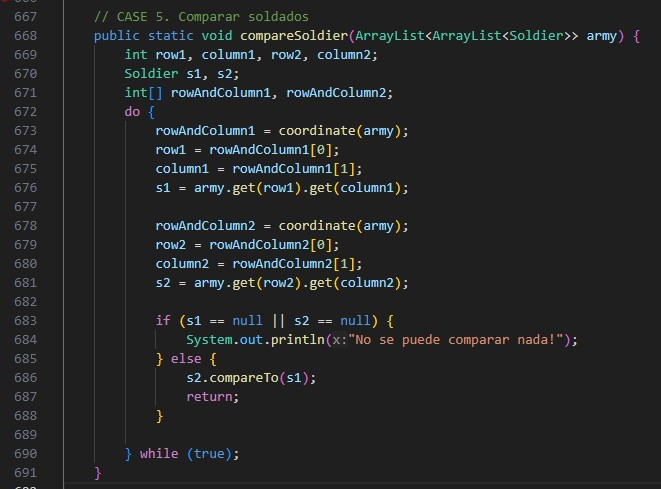
\includegraphics[width=1\textwidth,keepaspectratio]{img/compareSoldier.jpg}
		%\includesvg{img/automata.svg}
		%\label{img:mot2}
		%\caption{Product backlog.}
	\end{figure}
	
	\begin{itemize}	
		\item Este método se encarga de comparar los atributos de un Soldier, entre estos tenemos el nivel de vida actual, los puntos de ataque, defensa, estado (Si viven o no) y la velocidad.
	\end{itemize}
	
	\begin{lstlisting}[language=bash,caption={Compilando y probando el metodo compareSoldier  }][H]
		javac VideoJuego.java
		java VideoJuego
		1: Juego rapido
		2: Juego personalizado
		3: Salir
		2
		DATOS DEL EJRCITO A
		Soldier [name=Soldier1x2, row=1, column=2, attackLevel=2, defenseLevel=3, actualLife=5, speed=0, attitude=Repose, current=true]
		Soldier [name=Soldier2x6, row=2, column=6, attackLevel=5, defenseLevel=1, actualLife=2, speed=0, attitude=Repose, current=true]
		Soldier [name=Soldier4x9, row=4, column=9, attackLevel=5, defenseLevel=4, actualLife=4, speed=0, attitude=Repose, current=true]
		Soldier [name=Soldier7x9, row=7, column=9, attackLevel=4, defenseLevel=2, actualLife=4, speed=0, attitude=Repose, current=true]
		Soldier [name=Soldier10x10, row=10, column=10, attackLevel=1, defenseLevel=1, actualLife=3, speed=0, attitude=Repose, current=true]
		DATOS DEL EJRCITO B
		Soldier [name=Soldier5x4, row=5, column=4, attackLevel=2, defenseLevel=1, actualLife=5, speed=0, attitude=Repose, current=true]
		Soldier [name=Soldier5x7, row=5, column=7, attackLevel=2, defenseLevel=1, actualLife=1, speed=0, attitude=Repose, current=true]
		Soldier [name=Soldier7x8, row=7, column=8, attackLevel=2, defenseLevel=1, actualLife=4, speed=0, attitude=Repose, current=true]
		Soldier [name=Soldier8x4, row=8, column=4, attackLevel=2, defenseLevel=4, actualLife=4, speed=0, attitude=Repose, current=true]
		Soldier [name=Soldier8x6, row=8, column=6, attackLevel=1, defenseLevel=4, actualLife=2, speed=0, attitude=Repose, current=true]
		Soldier [name=Soldier9x8, row=9, column=8, attackLevel=2, defenseLevel=4, actualLife=3, speed=0, attitude=Repose, current=true]
		Soldier [name=Soldier10x3, row=10, column=3, attackLevel=2, defenseLevel=1, actualLife=4, speed=0, attitude=Repose, current=true]
		Soldier [name=Soldier10x6, row=10, column=6, attackLevel=1, defenseLevel=3, actualLife=1, speed=0, attitude=Repose, current=true]
		Soldier [name=Soldier10x7, row=10, column=7, attackLevel=4, defenseLevel=5, actualLife=5, speed=0, attitude=Repose, current=true]
		Soldier [name=Soldier10x8, row=10, column=8, attackLevel=5, defenseLevel=2, actualLife=3, speed=0, attitude=Repose, current=true]
		1: Crear soldado
		2: Eliminar soldado
		3: Clonar soldado
		4: Modificar soldado
		5: Comparar Soldado
		6: Intercambiar soldado
		7: Ver soldado
		8: Ver ejercito
		9: Sumar niveles
		10: Jugar
		11: Volver al menu principal
		5
		Elija el ejercito que editara:
		1: Ejercito A
		2: Ejercito B
		2
		Ingrese las coordenadas
		5d
		Ingrese las coordenadas
		10c
		Tienen igual nivel de ataque
		Tiene igual nivel de defensa
		Su vida actual son diferentes
		Ambos viven
		Tienen igual velocidad
		DATOS DEL EJRCITO A
		Soldier [name=Soldier1x2, row=1, column=2, attackLevel=2, defenseLevel=3, actualLife=5, speed=0, attitude=Repose, current=true]
		Soldier [name=Soldier2x6, row=2, column=6, attackLevel=5, defenseLevel=1, actualLife=2, speed=0, attitude=Repose, current=true]
		Soldier [name=Soldier4x9, row=4, column=9, attackLevel=5, defenseLevel=4, actualLife=4, speed=0, attitude=Repose, current=true]
		Soldier [name=Soldier7x9, row=7, column=9, attackLevel=4, defenseLevel=2, actualLife=4, speed=0, attitude=Repose, current=true]
		Soldier [name=Soldier10x10, row=10, column=10, attackLevel=1, defenseLevel=1, actualLife=3, speed=0, attitude=Repose, current=true]
		DATOS DEL EJRCITO B
		Soldier [name=Soldier5x4, row=5, column=4, attackLevel=2, defenseLevel=1, actualLife=5, speed=0, attitude=Repose, current=true]
		Soldier [name=Soldier5x7, row=5, column=7, attackLevel=2, defenseLevel=1, actualLife=1, speed=0, attitude=Repose, current=true]
		Soldier [name=Soldier7x8, row=7, column=8, attackLevel=2, defenseLevel=1, actualLife=4, speed=0, attitude=Repose, current=true]
		Soldier [name=Soldier8x4, row=8, column=4, attackLevel=2, defenseLevel=4, actualLife=4, speed=0, attitude=Repose, current=true]
		Soldier [name=Soldier8x6, row=8, column=6, attackLevel=1, defenseLevel=4, actualLife=2, speed=0, attitude=Repose, current=true]
		Soldier [name=Soldier9x8, row=9, column=8, attackLevel=2, defenseLevel=4, actualLife=3, speed=0, attitude=Repose, current=true]
		Soldier [name=Soldier10x3, row=10, column=3, attackLevel=2, defenseLevel=1, actualLife=4, speed=0, attitude=Repose, current=true]
		Soldier [name=Soldier10x6, row=10, column=6, attackLevel=1, defenseLevel=3, actualLife=1, speed=0, attitude=Repose, current=true]
		Soldier [name=Soldier10x7, row=10, column=7, attackLevel=4, defenseLevel=5, actualLife=5, speed=0, attitude=Repose, current=true]
		Soldier [name=Soldier10x8, row=10, column=8, attackLevel=5, defenseLevel=2, actualLife=3, speed=0, attitude=Repose, current=true]
		1: Crear soldado
		2: Eliminar soldado
		3: Clonar soldado
		4: Modificar soldado
		5: Comparar Soldado
		6: Intercambiar soldado
		7: Ver soldado
		8: Ver ejercito
		9: Sumar niveles
		10: Jugar
		11: Volver al menu principal
		11
		1: Juego rapido
		2: Juego personalizado
		3: Salir
		3
	\end{lstlisting}
	
	\begin{lstlisting}[language=bash,caption={Commit: 9d78c3620d8f037fa789e96d6367c1c0f8d2a075}][H]
		git add VideoJuego.java
		git commit -m "Se crea el metodo compareSoldier"			
		git push -u origin main
	\end{lstlisting}
	
	
	
	\begin{lstlisting}[language=bash,caption={Se implementa el método para intercambiar posiciones entre soldados }][H]
		code VideoJuego.java
	\end{lstlisting}
	
	\begin{figure}[H]
		\centering
		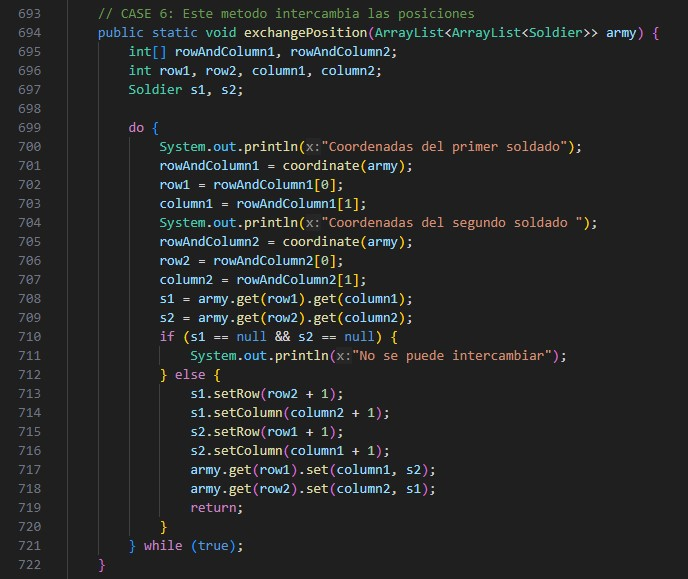
\includegraphics[width=1\textwidth,keepaspectratio]{img/exchangeSoldier.jpg}
		%\includesvg{img/automata.svg}
		%\label{img:mot2}
		%\caption{Product backlog.}
	\end{figure}
	
	\begin{itemize}	
		\item Este método se encarga de intercambiar la posición de dos Soldier del mismo ejército.
	\end{itemize}
	
	\begin{lstlisting}[language=bash,caption={Compilando y probando el metodo exchangeSoldier  }][H]
		javac VideoJuego.java
		java VideoJuego
		1: Juego rapido
		2: Juego personalizado
		3: Salir
		2
		DATOS DEL EJRCITO A
		Soldier [name=Soldier2x10, row=2, column=10, attackLevel=2, defenseLevel=2, actualLife=2, speed=0, attitude=Repose, current=true]
		Soldier [name=Soldier3x10, row=3, column=10, attackLevel=2, defenseLevel=3, actualLife=2, speed=0, attitude=Repose, current=true]
		Soldier [name=Soldier4x4, row=4, column=4, attackLevel=4, defenseLevel=5, actualLife=3, speed=0, attitude=Repose, current=true]
		Soldier [name=Soldier5x9, row=5, column=9, attackLevel=3, defenseLevel=3, actualLife=2, speed=0, attitude=Repose, current=true]
		Soldier [name=Soldier6x7, row=6, column=7, attackLevel=5, defenseLevel=1, actualLife=4, speed=0, attitude=Repose, current=true]
		Soldier [name=Soldier8x3, row=8, column=3, attackLevel=2, defenseLevel=4, actualLife=5, speed=0, attitude=Repose, current=true]
		Soldier [name=Soldier8x4, row=8, column=4, attackLevel=1, defenseLevel=1, actualLife=2, speed=0, attitude=Repose, current=true]
		Soldier [name=Soldier10x5, row=10, column=5, attackLevel=3, defenseLevel=2, actualLife=5, speed=0, attitude=Repose, current=true]
		Soldier [name=Soldier10x6, row=10, column=6, attackLevel=2, defenseLevel=5, actualLife=4, speed=0, attitude=Repose, current=true]
		DATOS DEL EJRCITO B
		Soldier [name=Soldier2x2, row=2, column=2, attackLevel=4, defenseLevel=3, actualLife=3, speed=0, attitude=Repose, current=true]
		Soldier [name=Soldier2x3, row=2, column=3, attackLevel=3, defenseLevel=3, actualLife=3, speed=0, attitude=Repose, current=true]
		Soldier [name=Soldier3x5, row=3, column=5, attackLevel=4, defenseLevel=5, actualLife=1, speed=0, attitude=Repose, current=true]
		Soldier [name=Soldier6x2, row=6, column=2, attackLevel=2, defenseLevel=5, actualLife=4, speed=0, attitude=Repose, current=true]
		Soldier [name=Soldier6x6, row=6, column=6, attackLevel=5, defenseLevel=3, actualLife=3, speed=0, attitude=Repose, current=true]
		Soldier [name=Soldier6x10, row=6, column=10, attackLevel=5, defenseLevel=4, actualLife=1, speed=0, attitude=Repose, current=true]
		Soldier [name=Soldier8x1, row=8, column=1, attackLevel=2, defenseLevel=4, actualLife=4, speed=0, attitude=Repose, current=true]
		Soldier [name=Soldier9x7, row=9, column=7, attackLevel=4, defenseLevel=3, actualLife=2, speed=0, attitude=Repose, current=true]
		Soldier [name=Soldier9x10, row=9, column=10, attackLevel=5, defenseLevel=2, actualLife=5, speed=0, attitude=Repose, current=true]
		Soldier [name=Soldier10x4, row=10, column=4, attackLevel=2, defenseLevel=4, actualLife=3, speed=0, attitude=Repose, current=true]
		1: Crear soldado
		2: Eliminar soldado
		3: Clonar soldado
		4: Modificar soldado
		5: Comparar Soldado
		6: Intercambiar soldado
		7: Ver soldado
		8: Ver ejercito
		9: Sumar niveles
		10: Jugar
		11: Volver al menu principal
		6
		Elija el ejercito que editara:
		1: Ejercito A
		2: Ejercito B
		1
		Coordenadas del primer soldado
		Ingrese las coordenadas
		2j
		Coordenadas del segundo soldado
		Ingrese las coordenadas
		3j
		DATOS DEL EJRCITO A
		Soldier [name=Soldier2x10, row=3, column=10, attackLevel=2, defenseLevel=2, actualLife=2, speed=0, attitude=Repose, current=true]
		Soldier [name=Soldier3x10, row=2, column=10, attackLevel=2, defenseLevel=3, actualLife=2, speed=0, attitude=Repose, current=true]
		Soldier [name=Soldier4x4, row=4, column=4, attackLevel=4, defenseLevel=5, actualLife=3, speed=0, attitude=Repose, current=true]
		Soldier [name=Soldier5x9, row=5, column=9, attackLevel=3, defenseLevel=3, actualLife=2, speed=0, attitude=Repose, current=true]
		Soldier [name=Soldier6x7, row=6, column=7, attackLevel=5, defenseLevel=1, actualLife=4, speed=0, attitude=Repose, current=true]
		Soldier [name=Soldier8x3, row=8, column=3, attackLevel=2, defenseLevel=4, actualLife=5, speed=0, attitude=Repose, current=true]
		Soldier [name=Soldier8x4, row=8, column=4, attackLevel=1, defenseLevel=1, actualLife=2, speed=0, attitude=Repose, current=true]
		Soldier [name=Soldier10x5, row=10, column=5, attackLevel=3, defenseLevel=2, actualLife=5, speed=0, attitude=Repose, current=true]
		Soldier [name=Soldier10x6, row=10, column=6, attackLevel=2, defenseLevel=5, actualLife=4, speed=0, attitude=Repose, current=true]
		DATOS DEL EJRCITO B
		Soldier [name=Soldier2x2, row=2, column=2, attackLevel=4, defenseLevel=3, actualLife=3, speed=0, attitude=Repose, current=true]
		Soldier [name=Soldier2x3, row=2, column=3, attackLevel=3, defenseLevel=3, actualLife=3, speed=0, attitude=Repose, current=true]
		Soldier [name=Soldier3x5, row=3, column=5, attackLevel=4, defenseLevel=5, actualLife=1, speed=0, attitude=Repose, current=true]
		Soldier [name=Soldier6x2, row=6, column=2, attackLevel=2, defenseLevel=5, actualLife=4, speed=0, attitude=Repose, current=true]
		Soldier [name=Soldier6x6, row=6, column=6, attackLevel=5, defenseLevel=3, actualLife=3, speed=0, attitude=Repose, current=true]
		Soldier [name=Soldier6x10, row=6, column=10, attackLevel=5, defenseLevel=4, actualLife=1, speed=0, attitude=Repose, current=true]
		Soldier [name=Soldier8x1, row=8, column=1, attackLevel=2, defenseLevel=4, actualLife=4, speed=0, attitude=Repose, current=true]
		Soldier [name=Soldier9x7, row=9, column=7, attackLevel=4, defenseLevel=3, actualLife=2, speed=0, attitude=Repose, current=true]
		Soldier [name=Soldier9x10, row=9, column=10, attackLevel=5, defenseLevel=2, actualLife=5, speed=0, attitude=Repose, current=true]
		Soldier [name=Soldier10x4, row=10, column=4, attackLevel=2, defenseLevel=4, actualLife=3, speed=0, attitude=Repose, current=true]
		1: Crear soldado
		2: Eliminar soldado
		3: Clonar soldado
		4: Modificar soldado
		5: Comparar Soldado
		6: Intercambiar soldado
		7: Ver soldado
		8: Ver ejercito
		9: Sumar niveles
		10: Jugar
		11: Volver al menu principal
		11
		1: Juego rapido
		2: Juego personalizado
		3: Salir
		3
	\end{lstlisting}
	
	\begin{lstlisting}[language=bash,caption={Commit: b825c23cde0e98518d0047f2867cb2a3f0d6fcf2}][H]
		git add VideoJuego.java
		git commit -m "Se implementa exchangePosition"			
		git push -u origin main
	\end{lstlisting}
	
	\begin{lstlisting}[language=bash,caption={Se implementa el método para intercambiar posiciones entre soldados }][H]
		code VideoJuego.java
	\end{lstlisting}
	
	\begin{figure}[H]
		\centering
		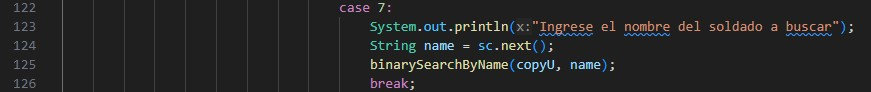
\includegraphics[width=1\textwidth,keepaspectratio]{img/searchSoldier.jpg}
		%\includesvg{img/automata.svg}
		%\label{img:mot2}
		%\caption{Product backlog.}
	\end{figure}
	
	\begin{itemize}	
		\item En el case 7 se implementa lo necesario para efectuar la búsqueda del Soldier que el usuario deseé. Se emplea la búsqueda binaria para tal propósito debido a su eficiencia.
	\end{itemize}
	
	\begin{lstlisting}[language=bash,caption={Compilando y probando el binarySearch  }][H]
		javac VideoJuego.java
		java VideoJuego
		1: Juego rapido
		2: Juego personalizado
		3: Salir
		2
		DATOS DEL EJRCITO A
		Soldier [name=Soldier4x5, row=4, column=5, attackLevel=3, defenseLevel=1, actualLife=3, speed=0, attitude=Repose, current=true]
		DATOS DEL EJRCITO B
		Soldier [name=Soldier4x9, row=4, column=9, attackLevel=1, defenseLevel=5, actualLife=1, speed=0, attitude=Repose, current=true]
		Soldier [name=Soldier6x1, row=6, column=1, attackLevel=1, defenseLevel=4, actualLife=1, speed=0, attitude=Repose, current=true]
		1: Crear soldado
		2: Eliminar soldado
		3: Clonar soldado
		4: Modificar soldado
		5: Comparar Soldado
		6: Intercambiar soldado
		7: Ver soldado
		8: Ver ejercito
		9: Sumar niveles
		10: Jugar
		11: Volver al menu principal
		7
		Elija el ejercito que editara:
		1: Ejercito A
		2: Ejercito B
		1
		Ingrese el nombre del soldado a buscar
		soldier4x5
		Se ha encontrado: Soldier [name=Soldier4x5, row=4, column=5, attackLevel=3, defenseLevel=1, actualLife=3, speed=0, attitude=Repose, current=true]
		DATOS DEL EJRCITO A
		Soldier [name=Soldier4x5, row=4, column=5, attackLevel=3, defenseLevel=1, actualLife=3, speed=0, attitude=Repose, current=true]
		DATOS DEL EJRCITO B
		Soldier [name=Soldier4x9, row=4, column=9, attackLevel=1, defenseLevel=5, actualLife=1, speed=0, attitude=Repose, current=true]
		Soldier [name=Soldier6x1, row=6, column=1, attackLevel=1, defenseLevel=4, actualLife=1, speed=0, attitude=Repose, current=true]
		1: Crear soldado
		2: Eliminar soldado
		3: Clonar soldado
		4: Modificar soldado
		5: Comparar Soldado
		6: Intercambiar soldado
		7: Ver soldado
		8: Ver ejercito
		9: Sumar niveles
		10: Jugar
	\end{lstlisting}
	
	
	
	
	
	
	
	\begin{lstlisting}[language=bash,caption={Se implementa el método para sumar los atributos de un ArrayList de Soldier }][H]
		code VideoJuego.java
	\end{lstlisting}
	
	\begin{figure}[H]
		\centering
		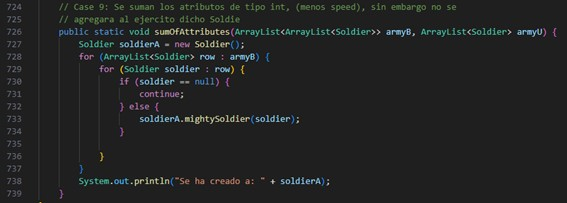
\includegraphics[width=1\textwidth,keepaspectratio]{img/sumAttributes.jpg}
		%\includesvg{img/automata.svg}
		%\label{img:mot2}
		%\caption{Product backlog.}
	\end{figure}
	
	\begin{itemize}	
		\item Este método se encarga de sumar los atributos de tipo int de un ArrayList de Soldier. Para lograr este cometido, debemos crear un Soldier cuyos atributos de tipo int sean iniciados en 0, por eso en la clase Soldier se creó un constructor que no admitía parámetros, pero cuyos valores ya eran inicializados en 0. Se usará dicho Soldier como un acumulador, ya que recordemos que cuando usamos métodos en objetos, lo que se pasa y se modifica es la referencia en si, por lo que en cada iteración los valores sumados de los atributos se irán acumulando en el Soldier creado.
	\end{itemize}
	
	\begin{lstlisting}[language=bash,caption={Compilando y probando el metodo sumOfAttributes  }][H]
		javac VideoJuego.java
		java VideoJuego
		1: Juego rapido
		2: Juego personalizado
		3: Salir
		2
		DATOS DEL EJRCITO A
		Soldier [name=Soldier2x5, row=2, column=5, attackLevel=5, defenseLevel=5, actualLife=5, speed=0, attitude=Repose, current=true]
		Soldier [name=Soldier3x7, row=3, column=7, attackLevel=1, defenseLevel=5, actualLife=5, speed=0, attitude=Repose, current=true]
		Soldier [name=Soldier4x10, row=4, column=10, attackLevel=3, defenseLevel=3, actualLife=5, speed=0, attitude=Repose, current=true]
		DATOS DEL EJRCITO B
		Soldier [name=Soldier5x4, row=5, column=4, attackLevel=4, defenseLevel=3, actualLife=4, speed=0, attitude=Repose, current=true]
		Soldier [name=Soldier8x1, row=8, column=1, attackLevel=1, defenseLevel=4, actualLife=4, speed=0, attitude=Repose, current=true]
		Soldier [name=Soldier8x8, row=8, column=8, attackLevel=4, defenseLevel=4, actualLife=5, speed=0, attitude=Repose, current=true]
		Soldier [name=Soldier10x3, row=10, column=3, attackLevel=4, defenseLevel=2, actualLife=3, speed=0, attitude=Repose, current=true]
		1: Crear soldado
		2: Eliminar soldado
		3: Clonar soldado
		4: Modificar soldado
		5: Comparar Soldado
		6: Intercambiar soldado
		7: Ver soldado
		8: Ver ejercito
		9: Sumar niveles
		10: Jugar
		11: Volver al menu principal
		9
		Elija el ejercito que editara:
		1: Ejercito A
		2: Ejercito B
		1
		Se ha creado a: Soldier [name=NotFound, row=0, column=0, attackLevel=9, defenseLevel=13, actualLife=15, speed=0, attitude=repose, current=true]
		DATOS DEL EJRCITO A
		Soldier [name=Soldier2x5, row=2, column=5, attackLevel=5, defenseLevel=5, actualLife=5, speed=0, attitude=Repose, current=true]
		Soldier [name=Soldier3x7, row=3, column=7, attackLevel=1, defenseLevel=5, actualLife=5, speed=0, attitude=Repose, current=true]
		Soldier [name=Soldier4x10, row=4, column=10, attackLevel=3, defenseLevel=3, actualLife=5, speed=0, attitude=Repose, current=true]
		DATOS DEL EJRCITO B
		Soldier [name=Soldier5x4, row=5, column=4, attackLevel=4, defenseLevel=3, actualLife=4, speed=0, attitude=Repose, current=true]
		Soldier [name=Soldier8x1, row=8, column=1, attackLevel=1, defenseLevel=4, actualLife=4, speed=0, attitude=Repose, current=true]
		Soldier [name=Soldier8x8, row=8, column=8, attackLevel=4, defenseLevel=4, actualLife=5, speed=0, attitude=Repose, current=true]
		Soldier [name=Soldier10x3, row=10, column=3, attackLevel=4, defenseLevel=2, actualLife=3, speed=0, attitude=Repose, current=true]
		1: Crear soldado
		2: Eliminar soldado
		3: Clonar soldado
		4: Modificar soldado
		5: Comparar Soldado
		6: Intercambiar soldado
		7: Ver soldado
		8: Ver ejercito
		9: Sumar niveles
		10: Jugar
		11: Volver al menu principal
		11
		1: Juego rapido
		2: Juego personalizado
		3: Salir
		3
	\end{lstlisting}
	
	\begin{lstlisting}[language=bash,caption={Commit: ccb448aabe0c75743e18946a8e2965bc9790ce37}][H]
		git add VideoJuego.java
		git commit -m "Se crea el metodo sumOfAttribute"			
		git push -u origin main
	\end{lstlisting}
	
	
	
	
	
	
	
	
	
	
	
	
	
	\begin{lstlisting}[language=bash,caption={Se implementa el método de batalla rápida}][H]
		code VideoJuego.java
	\end{lstlisting}
	
	\begin{figure}[H]
		\centering
		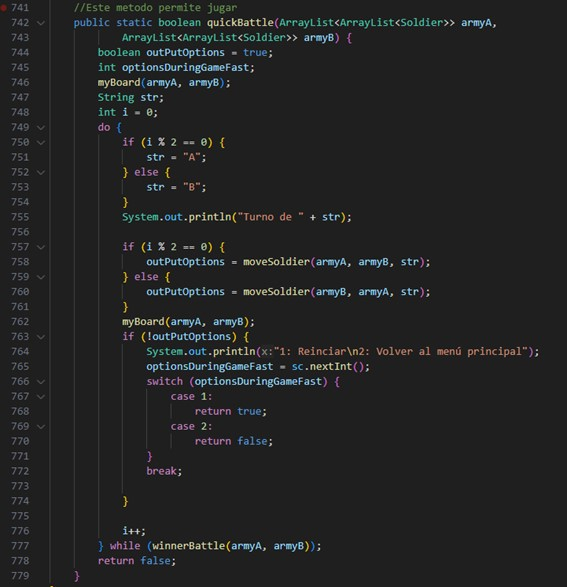
\includegraphics[width=0.9\textwidth,keepaspectratio]{img/quickBattle.jpg}
		%\includesvg{img/automata.svg}
		%\label{img:mot2}
		%\caption{Product backlog.}
	\end{figure}
	
	\begin{itemize}	
		\item Este método se encarga de poder jugar. En este método se usan los método moveSoldier el cual permite desplazarnos casilla por casilla y el método winnerBattle el cual detiene el flujo del programa arrojando un mensaje indicando el ganador. Este método retorna booleanos porque esto nos indica si el usuario decidió cancelar la partida o no.
	\end{itemize}
	
	\begin{lstlisting}[language=bash,caption={Compilando y probando el programa completo  }][H]
		javac VideoJuego.java
		java VideoJuego
		1: Juego rapido
		2: Juego personalizado
		3: Salir
		2
		DATOS DEL EJRCITO A
		Soldier [name=Soldier6x2, row=6, column=2, attackLevel=1, defenseLevel=5, actualLife=1, speed=0, attitude=Repose, current=true]
		DATOS DEL EJRCITO B
		Soldier [name=Soldier1x4, row=1, column=4, attackLevel=3, defenseLevel=3, actualLife=4, speed=0, attitude=Repose, current=true]
		Soldier [name=Soldier6x4, row=6, column=4, attackLevel=1, defenseLevel=4, actualLife=2, speed=0, attitude=Repose, current=true]
		Soldier [name=Soldier7x6, row=7, column=6, attackLevel=4, defenseLevel=2, actualLife=1, speed=0, attitude=Repose, current=true]
		Soldier [name=Soldier7x7, row=7, column=7, attackLevel=1, defenseLevel=4, actualLife=4, speed=0, attitude=Repose, current=true]
		Soldier [name=Soldier9x5, row=9, column=5, attackLevel=2, defenseLevel=5, actualLife=1, speed=0, attitude=Repose, current=true]
		Soldier [name=Soldier10x2, row=10, column=2, attackLevel=1, defenseLevel=3, actualLife=2, speed=0, attitude=Repose, current=true]
		1: Crear soldado
		2: Eliminar soldado
		3: Clonar soldado
		4: Modificar soldado
		5: Comparar Soldado
		6: Intercambiar soldado
		7: Ver soldado
		8: Ver ejercito
		9: Sumar niveles
		10: Jugar
		11: Volver al menu principal
		2
		Elija el ejercito que editara:
		1: Ejercito A
		2: Ejercito B
		2
		Debe Eliminar un soldado
		    	A     B     C      D      E     F      G      H      I     J 
		1 |____||____||____||_b4_||____||____||____||____||____||____|
		2 |____||____||____||____||____||____||____||____||____||____|
		3 |____||____||____||____||____||____||____||____||____||____|
		4 |____||____||____||____||____||____||____||____||____||____|
		5 |____||____||____||____||____||____||____||____||____||____|
		6 |____||_a1_||____||_b2_||____||____||____||____||____||____|
		7 |____||____||____||____||____||_b1_||_b4_||____||____||____|
		8 |____||____||____||____||____||____||____||____||____||____|
		9 |____||____||____||____||_b1_||____||____||____||____||____|
		10|____||_b2_||____||____||____||____||____||____||____||____|
		Soldier [name=Soldier1x4, row=1, column=4, attackLevel=3, defenseLevel=3, actualLife=4, speed=0, attitude=Repose, current=true]
		Soldier [name=Soldier6x4, row=6, column=4, attackLevel=1, defenseLevel=4, actualLife=2, speed=0, attitude=Repose, current=true]
		Soldier [name=Soldier7x6, row=7, column=6, attackLevel=4, defenseLevel=2, actualLife=1, speed=0, attitude=Repose, current=true]
		Soldier [name=Soldier7x7, row=7, column=7, attackLevel=1, defenseLevel=4, actualLife=4, speed=0, attitude=Repose, current=true]
		Soldier [name=Soldier9x5, row=9, column=5, attackLevel=2, defenseLevel=5, actualLife=1, speed=0, attitude=Repose, current=true]
		Soldier [name=Soldier10x2, row=10, column=2, attackLevel=1, defenseLevel=3, actualLife=2, speed=0, attitude=Repose, current=true]
		Ingrese las coordenadas
		10b
		DATOS DEL EJRCITO A
		Soldier [name=Soldier6x2, row=6, column=2, attackLevel=1, defenseLevel=5, actualLife=1, speed=0, attitude=Repose, current=true]
		DATOS DEL EJRCITO B
		Soldier [name=Soldier1x4, row=1, column=4, attackLevel=3, defenseLevel=3, actualLife=4, speed=0, attitude=Repose, current=true]
		Soldier [name=Soldier6x4, row=6, column=4, attackLevel=1, defenseLevel=4, actualLife=2, speed=0, attitude=Repose, current=true]
		Soldier [name=Soldier7x6, row=7, column=6, attackLevel=4, defenseLevel=2, actualLife=1, speed=0, attitude=Repose, current=true]
		Soldier [name=Soldier7x7, row=7, column=7, attackLevel=1, defenseLevel=4, actualLife=4, speed=0, attitude=Repose, current=true]
		Soldier [name=Soldier9x5, row=9, column=5, attackLevel=2, defenseLevel=5, actualLife=1, speed=0, attitude=Repose, current=true]
		1: Crear soldado
		2: Eliminar soldado
		3: Clonar soldado
		4: Modificar soldado
		5: Comparar Soldado
		6: Intercambiar soldado
		7: Ver soldado
		8: Ver ejercito
		9: Sumar niveles
		10: Jugar
		11: Volver al menu principal
		1
		Elija el ejercito que editara:
		1: Ejercito A
		2: Ejercito B
		2
		Ingrese la fila (ejm 1,2,3..10)
		6
		Ingrese la columna (ejm 1,2,3...10)
		1
		Ingrese el nivel de ataque
		5
		Ingrese el nivel de defensa
		5
		Ingrese el nivel de vida
		5
		Ingrese la velocidad
		5
		DATOS DEL EJRCITO A
		Soldier [name=Soldier6x2, row=6, column=2, attackLevel=1, defenseLevel=5, actualLife=1, speed=0, attitude=Repose, current=true]
		DATOS DEL EJRCITO B
		Soldier [name=Soldier1x4, row=1, column=4, attackLevel=3, defenseLevel=3, actualLife=4, speed=0, attitude=Repose, current=true]
		Soldier [name=Soldier6x4, row=6, column=4, attackLevel=1, defenseLevel=4, actualLife=2, speed=0, attitude=Repose, current=true]
		Soldier [name=Soldier7x6, row=7, column=6, attackLevel=4, defenseLevel=2, actualLife=1, speed=0, attitude=Repose, current=true]
		Soldier [name=Soldier7x7, row=7, column=7, attackLevel=1, defenseLevel=4, actualLife=4, speed=0, attitude=Repose, current=true]
		Soldier [name=Soldier9x5, row=9, column=5, attackLevel=2, defenseLevel=5, actualLife=1, speed=0, attitude=Repose, current=true]
		Soldier [name=Soldier6X1, row=6, column=1, attackLevel=5, defenseLevel=5, actualLife=5, speed=0, attitude=Repose, current=true]
		1: Crear soldado
		2: Eliminar soldado
		3: Clonar soldado
		4: Modificar soldado
		5: Comparar Soldado
		6: Intercambiar soldado
		7: Ver soldado
		8: Ver ejercito
		9: Sumar niveles
		10: Jugar
		11: Volver al menu principal
		10
		Elija el ejercito que editara:
		1: Ejercito A
		2: Ejercito B
		1
		oooooooooooooooo  FASE 1 DE LA CONTIENDA  oooooooooooooooo
		Mostrando estadisticas de cada ejercito
		
		DATOS DEL DEL EJERCITO A
		Soldier [name=Soldier6x2, row=6, column=2, attackLevel=1, defenseLevel=5, actualLife=1, speed=0, attitude=Repose, current=true]
		DATOS DEL EJRCITO B
		Soldier [name=Soldier1x4, row=1, column=4, attackLevel=3, defenseLevel=3, actualLife=4, speed=0, attitude=Repose, current=true]
		Soldier [name=Soldier6x4, row=6, column=4, attackLevel=1, defenseLevel=4, actualLife=2, speed=0, attitude=Repose, current=true]
		Soldier [name=Soldier7x6, row=7, column=6, attackLevel=4, defenseLevel=2, actualLife=1, speed=0, attitude=Repose, current=true]
		Soldier [name=Soldier7x7, row=7, column=7, attackLevel=1, defenseLevel=4, actualLife=4, speed=0, attitude=Repose, current=true]
		Soldier [name=Soldier9x5, row=9, column=5, attackLevel=2, defenseLevel=5, actualLife=1, speed=0, attitude=Repose, current=true]
		Soldier [name=Soldier6X1, row=6, column=1, attackLevel=5, defenseLevel=5, actualLife=5, speed=0, attitude=Repose, current=true]
		
		oooooooooooooooo  FASE 2 DE LA CONTIENDA  oooooooooooooooo
		Mostrando el tablero de juego
			A     B     C      D      E     F      G      H      I     J 
		1 |____||____||____||_b4_||____||____||____||____||____||____|
		2 |____||____||____||____||____||____||____||____||____||____|
		3 |____||____||____||____||____||____||____||____||____||____|
		4 |____||____||____||____||____||____||____||____||____||____|
		5 |____||____||____||____||____||____||____||____||____||____|
		6 |_b5_||_a1_||____||_b2_||____||____||____||____||____||____|
		7 |____||____||____||____||____||_b1_||_b4_||____||____||____|
		8 |____||____||____||____||____||____||____||____||____||____|
		9 |____||____||____||____||_b1_||____||____||____||____||____|
		10|____||____||____||____||____||____||____||____||____||____|
		
		+++++++++++++++++   FASE 3 DE LA CONTIENDA  +++++++++++++++++
			 A     B     C      D      E     F      G      H      I     J 
		1 |____||____||____||_b4_||____||____||____||____||____||____|
		2 |____||____||____||____||____||____||____||____||____||____|
		3 |____||____||____||____||____||____||____||____||____||____|
		4 |____||____||____||____||____||____||____||____||____||____|
		5 |____||____||____||____||____||____||____||____||____||____|
		6 |_b5_||_a1_||____||_b2_||____||____||____||____||____||____|
		7 |____||____||____||____||____||_b1_||_b4_||____||____||____|
		8 |____||____||____||____||____||____||____||____||____||____|
		9 |____||____||____||____||_b1_||____||____||____||____||____|
		10|____||____||____||____||____||____||____||____||____||____|
		Turno de A
		Ingrese las coordenadas
		6b
		Hacia donde quiere mover? up(1), down(2), left(3), right(4), exit(5)
		3
		Estadisticas de batalla:        Soldado de atacante: 16.666666666666668%        Soldado en reposo: 83.33333333333333    Salio como aleatorio: 82.79657290860615
		Soldier [name=Soldier6X1, row=6, column=1, attackLevel=5, defenseLevel=5, actualLife=5, speed=2, attitude=offensive, current=true]
		Soldier [name=Soldier6x2, row=6, column=2, attackLevel=1, defenseLevel=5, actualLife=1, speed=1, attitude=offensive, current=true]
		Ha ganado el soldado en reposo
		Soldier [name=Soldier6x2, row=6, column=2, attackLevel=1, defenseLevel=5, actualLife=1, speed=1, attitude=offensive, current=true]
			 A     B     C      D      E     F      G      H      I     J 
		1 |____||____||____||_b4_||____||____||____||____||____||____|
		2 |____||____||____||____||____||____||____||____||____||____|
		3 |____||____||____||____||____||____||____||____||____||____|
		4 |____||____||____||____||____||____||____||____||____||____|
		5 |____||____||____||____||____||____||____||____||____||____|
		6 |_b5_||____||____||_b2_||____||____||____||____||____||____|
		7 |____||____||____||____||____||_b1_||_b4_||____||____||____|
		8 |____||____||____||____||____||____||____||____||____||____|
		9 |____||____||____||____||_b1_||____||____||____||____||____|
		10|____||____||____||____||____||____||____||____||____||____|
		Ha ganado B
		DATOS DEL EJRCITO A
		Soldier [name=Soldier6x2, row=6, column=2, attackLevel=1, defenseLevel=5, actualLife=1, speed=1, attitude=offensive, current=true]
		DATOS DEL EJRCITO B
		Soldier [name=Soldier1x4, row=1, column=4, attackLevel=3, defenseLevel=3, actualLife=4, speed=0, attitude=Repose, current=true]
		Soldier [name=Soldier6x4, row=6, column=4, attackLevel=1, defenseLevel=4, actualLife=2, speed=0, attitude=Repose, current=true]
		Soldier [name=Soldier7x6, row=7, column=6, attackLevel=4, defenseLevel=2, actualLife=1, speed=0, attitude=Repose, current=true]
		Soldier [name=Soldier7x7, row=7, column=7, attackLevel=1, defenseLevel=4, actualLife=4, speed=0, attitude=Repose, current=true]
		Soldier [name=Soldier9x5, row=9, column=5, attackLevel=2, defenseLevel=5, actualLife=1, speed=0, attitude=Repose, current=true]
		Soldier [name=Soldier6X1, row=6, column=1, attackLevel=5, defenseLevel=5, actualLife=5, speed=2, attitude=offensive, current=true]
		1: Crear soldado
		2: Eliminar soldado
		3: Clonar soldado
		4: Modificar soldado
		5: Comparar Soldado
		6: Intercambiar soldado
		7: Ver soldado
		8: Ver ejercito
		9: Sumar niveles
		10: Jugar
		11: Volver al menu principal
		11
		1: Juego rapido
		2: Juego personalizado
		3: Salir
		1
		Desea jugar una ronda?(si/no)
		si
		oooooooooooooooo  FASE 1 DE LA CONTIENDA  oooooooooooooooo
		Mostrando estadisticas de cada ejercito
		
		DATOS DEL DEL EJERCITO A
		Soldier [name=Soldier5x1, row=5, column=1, attackLevel=5, defenseLevel=1, actualLife=2, speed=0, attitude=Repose, current=true]
		Soldier [name=Soldier8x5, row=8, column=5, attackLevel=5, defenseLevel=4, actualLife=5, speed=0, attitude=Repose, current=true]
		DATOS DEL EJRCITO B
		Soldier [name=Soldier4x1, row=4, column=1, attackLevel=1, defenseLevel=3, actualLife=1, speed=0, attitude=Repose, current=true]
		Soldier [name=Soldier4x5, row=4, column=5, attackLevel=2, defenseLevel=2, actualLife=2, speed=0, attitude=Repose, current=true]
		Soldier [name=Soldier5x5, row=5, column=5, attackLevel=1, defenseLevel=5, actualLife=3, speed=0, attitude=Repose, current=true]
		Soldier [name=Soldier6x5, row=6, column=5, attackLevel=1, defenseLevel=2, actualLife=2, speed=0, attitude=Repose, current=true]
		Soldier [name=Soldier7x9, row=7, column=9, attackLevel=2, defenseLevel=4, actualLife=1, speed=0, attitude=Repose, current=true]
		
		oooooooooooooooo  FASE 2 DE LA CONTIENDA  oooooooooooooooo
		Mostrando el tablero de juego
			 A     B     C      D      E     F      G      H      I     J 
		1 |____||____||____||____||____||____||____||____||____||____|
		2 |____||____||____||____||____||____||____||____||____||____|
		3 |____||____||____||____||____||____||____||____||____||____|
		4 |_b1_||____||____||____||_b2_||____||____||____||____||____|
		5 |_a2_||____||____||____||_b3_||____||____||____||____||____|
		6 |____||____||____||____||_b2_||____||____||____||____||____|
		7 |____||____||____||____||____||____||____||____||_b1_||____|
		8 |____||____||____||____||_a5_||____||____||____||____||____|
		9 |____||____||____||____||____||____||____||____||____||____|
		10|____||____||____||____||____||____||____||____||____||____|
		
		+++++++++++++++++   FASE 3 DE LA CONTIENDA  +++++++++++++++++
			 A     B     C      D      E     F      G      H      I     J 
		1 |____||____||____||____||____||____||____||____||____||____|
		2 |____||____||____||____||____||____||____||____||____||____|
		3 |____||____||____||____||____||____||____||____||____||____|
		4 |_b1_||____||____||____||_b2_||____||____||____||____||____|
		5 |_a2_||____||____||____||_b3_||____||____||____||____||____|
		6 |____||____||____||____||_b2_||____||____||____||____||____|
		7 |____||____||____||____||____||____||____||____||_b1_||____|
		8 |____||____||____||____||_a5_||____||____||____||____||____|
		9 |____||____||____||____||____||____||____||____||____||____|
		10|____||____||____||____||____||____||____||____||____||____|
		Turno de A
		Ingrese las coordenadas
		salir
			 A     B     C      D      E     F      G      H      I     J 
		1 |____||____||____||____||____||____||____||____||____||____|
		2 |____||____||____||____||____||____||____||____||____||____|
		3 |____||____||____||____||____||____||____||____||____||____|
		4 |_b1_||____||____||____||_b2_||____||____||____||____||____|
		5 |_a2_||____||____||____||_b3_||____||____||____||____||____|
		6 |____||____||____||____||_b2_||____||____||____||____||____|
		7 |____||____||____||____||____||____||____||____||_b1_||____|
		8 |____||____||____||____||_a5_||____||____||____||____||____|
		9 |____||____||____||____||____||____||____||____||____||____|
		10|____||____||____||____||____||____||____||____||____||____|
		1: Reinciar
		2: Volver al menu principal
		2
		1: Juego rapido
		2: Juego personalizado
		3: Salir
		3
	\end{lstlisting}
	
	\begin{lstlisting}[language=bash,caption={Commit: a2ccc9dec857e9f4649ee5e6729ac4f3194ffb7d}][H]
		git add VideoJuego.java
		git commit -m "Metodo quickBattle terminado"			
		git push -u origin main
	\end{lstlisting}
	
	
	
	
	
	
	
	
	
	\subsection{Diagrama UML}
	
	\begin{figure}[H]
		\centering
		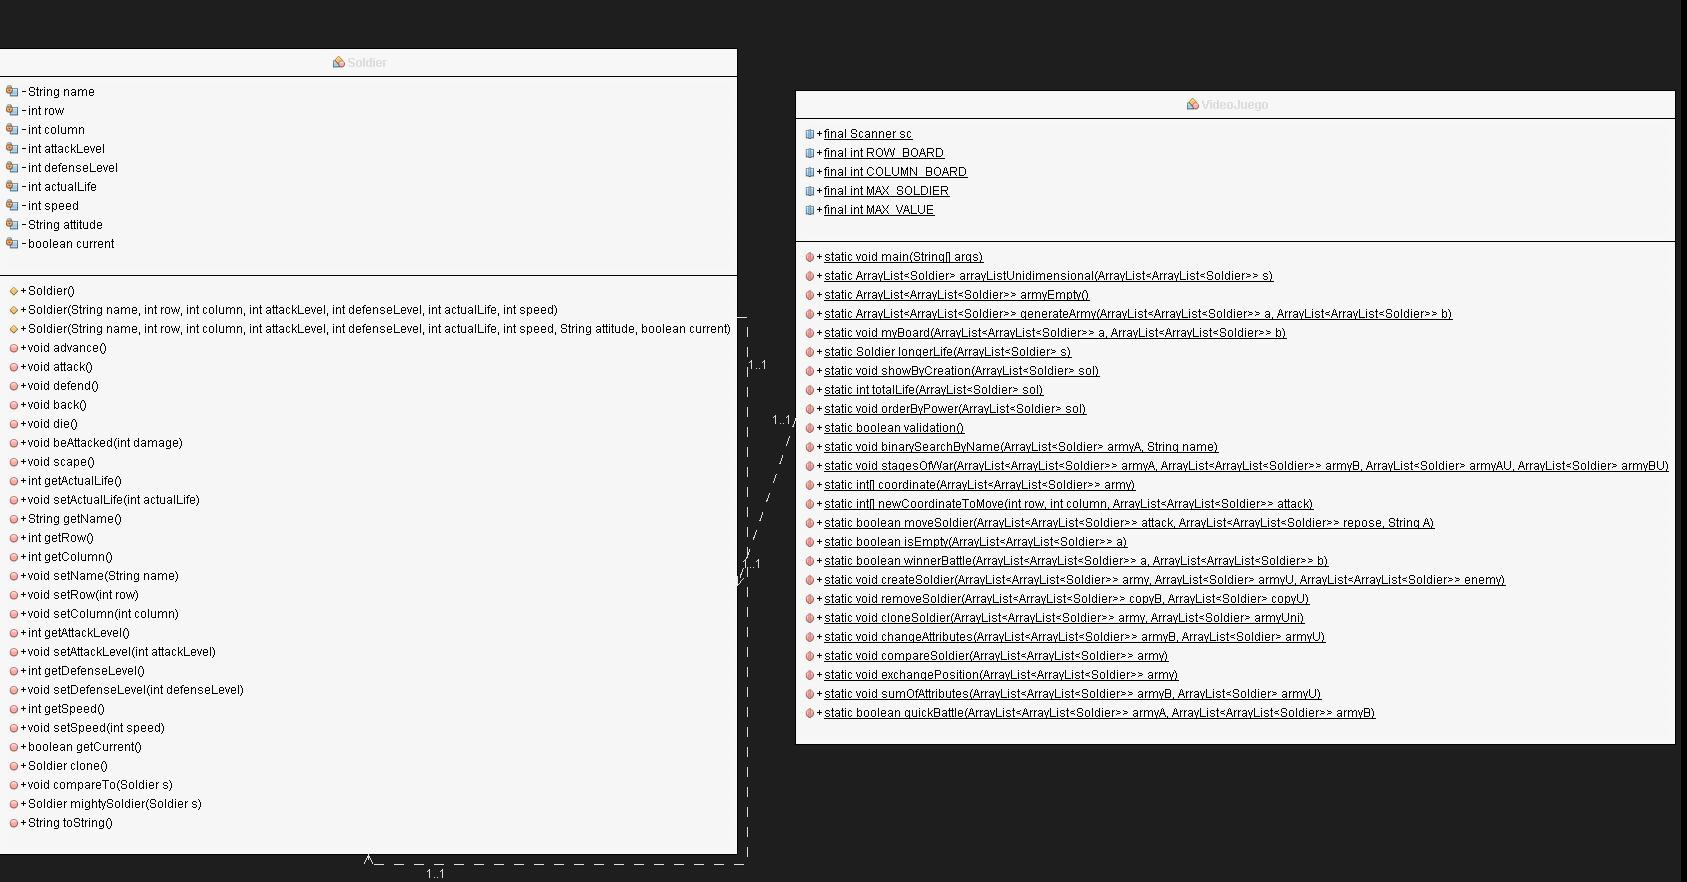
\includegraphics[width=1\textwidth,keepaspectratio]{img/uml.png}
		%\includesvg{img/automata.svg}
		%\label{img:mot2}
		%\caption{Product backlog.}
	\end{figure}
	
	
	\subsection{Estructura de laboratorio 12}
	\begin{itemize}	
		\item El contenido que se entrega en este laboratorio es el siguiente:
	\end{itemize}
	
	\begin{lstlisting}[style=ascii-tree]
		lab12:
		|   Soldier.java
		|   VideoJuego.java
		|
		 ---latex
			 |   programacion_lab12_rescobedoq_v1.0.pdf
			 |   programacion_lab12_rescobedoq_v1.0.tex
			 |
			  ---img
						armyEmpty.jpg
						arrayListU.jpg
						binary.jpg
						binarySearchByName.jpg
						burbuja.jpg
						changeAttribute.jpg
						changesMyBoard.jpg
						classSoldier.jpg
						clone.jpg
						cloneSoldier.jpg
						compare.jpg
						compareSoldier.jpg
						constructors.jpg
						coordinate.jpg
						copyReference.jpg
						createSoldier.jpg
						exchangeSoldier.jpg
						generateArmy.jpg
						generateUni.jpg
						insertion.jpg
						isEmpty.jpg
						logo_abet.png
						logo_episunsa.png
						logo_unsa.jpg
						longerLife.jpg
						method.jpg
						method2.jpg
						method3.jpg
						method4.jpg
						mightySoldier.jpg
						moveSoldier.jpg
						myBoard.jpg
						newCoordinate.jpg
						orderByPower.png
						quickBattle.jpg
						removeSoldier.jpg
						searchSoldier.jpg
						sequence.jpg
						showByCreation.jpg
						stages.jpg
						sumAttributes.jpg
						toString.jpg
						totalLife.jpg
						uml.png
						validation.jpg
						winnerBattle.png
			
	\end{lstlisting}    
	
	\section{\textcolor{red}{Rúbricas}}
	
	\subsection{\textcolor{red}{Entregable Informe}}
	\begin{table}[H]
		\caption{Tipo de Informe}
		\setlength{\tabcolsep}{0.5em} % for the horizontal padding
		{\renewcommand{\arraystretch}{1.5}% for the vertical padding
			\begin{tabular}{|p{3cm}|p{12cm}|}
				\hline
				\multicolumn{2}{|c|}{\textbf{\textcolor{red}{Informe}}}  \\
				\hline 
				\textbf{\textcolor{red}{Latex}} & \textcolor{blue}{El informe está en formato PDF desde Latex,  con un formato limpio (buena presentación) y facil de leer.}   \\ 
				\hline 
				
				
			\end{tabular}
		}
	\end{table}
	
	\clearpage
	
	\subsection{\textcolor{red}{Rúbrica para el contenido del Informe y demostración}}
	\begin{itemize}			
		\item El alumno debe marcar o dejar en blanco en celdas de la columna \textbf{Checklist} si cumplio con el ítem correspondiente.
		\item Si un alumno supera la fecha de entrega,  su calificación será sobre la nota mínima aprobada, siempre y cuando cumpla con todos lo items.
		\item El alumno debe autocalificarse en la columna \textbf{Estudiante} de acuerdo a la siguiente tabla:
		
		\begin{table}[ht]
			\caption{Niveles de desempeño}
			\begin{center}
				\begin{tabular}{ccccc}
					\hline
					& \multicolumn{4}{c}{Nivel}\\
					\cline{1-5}
					\textbf{Puntos} & Insatisfactorio 25\%& En Proceso 50\% & Satisfactorio 75\% & Sobresaliente 100\%\\
					\textbf{2.0}&0.5&1.0&1.5&2.0\\
					\textbf{4.0}&1.0&2.0&3.0&4.0\\
					\hline
				\end{tabular}
			\end{center}
		\end{table}	
		
	\end{itemize}
	
	\begin{table}[H]
		\caption{Rúbrica para contenido del Informe y demostración}
		\setlength{\tabcolsep}{0.5em} % for the horizontal padding
		{\renewcommand{\arraystretch}{1.5}% for the vertical padding
			%\begin{center}
			\begin{tabular}{|p{2.7cm}|p{7cm}|x{1.3cm}|p{1.2cm}|p{1.5cm}|p{1.1cm}|}
				\hline
				\multicolumn{2}{|c|}{Contenido y demostración} & Puntos & Checklist & Estudiante & Profesor\\
				\hline
				\textbf{1. GitHub} & Hay enlace URL activo del directorio para el  laboratorio hacia su repositorio GitHub con código fuente terminado y fácil de revisar. &2 &X &2 & \\ 
				\hline
				\textbf{2. Commits} &  Hay capturas de pantalla de los commits más importantes con sus explicaciones detalladas. (El profesor puede preguntar para refrendar calificación). &4 &X &4 & \\ 
				\hline 
				\textbf{3. Código fuente} &  Hay porciones de código fuente importantes con numeración y explicaciones detalladas de sus funciones. &2 &X &2 & \\ 
				\hline 
				\textbf{4. Ejecución} & Se incluyen ejecuciones/pruebas del código fuente  explicadas gradualmente. &2 &X &2 & \\ 
				\hline			
				\textbf{5. Pregunta} & Se responde con completitud a la pregunta formulada en la tarea.  (El profesor puede preguntar para refrendar calificación).  &2 &X &2 & \\ 
				\hline	
				\textbf{6. Fechas} & Las fechas de modificación del código fuente estan dentro de los plazos de fecha de entrega establecidos. &2 &X &2 & \\ 
				\hline 
				\textbf{7. Ortografía} & El documento no muestra errores ortográficos. &2 &X &2 & \\ 
				\hline 
				\textbf{8. Madurez} & El Informe muestra de manera general una evolución de la madurez del código fuente,  explicaciones puntuales pero precisas y un acabado impecable.   (El profesor puede preguntar para refrendar calificación).  &4 &X &2 & \\ 
				\hline
				\multicolumn{2}{|c|}{\textbf{Total}} &20 & &18 & \\ 
				\hline
			\end{tabular}
			%\end{center}
			%\label{tab:multicol}
		}
	\end{table}
	
	\clearpage
	
	\section{Referencias}
	\begin{itemize}			
		\item \url{https://www.geeksforgeeks.org/binary-search/}
		\item \url{https://www.geeksforgeeks.org/insertion-sort/}
	\end{itemize}	
	
	%\clearpage
	%\bibliographystyle{apalike}
	%\bibliographystyle{IEEEtranN}
	%\bibliography{bibliography}
	
\end{document}